\documentclass[a4paper]{llncs}

%\documentclass{llncs}
%
\usepackage[T1]{fontenc}
\usepackage{lmodern}
\usepackage[utf8]{inputenc}
\usepackage{amsfonts}
\usepackage{amsmath}
\usepackage{amssymb}
\usepackage{booktabs}
\usepackage{makeidx}  % allows for indexgeneration
%
\usepackage{epsfig} 
\usepackage[ruled,vlined,linesnumbered]{algorithm2e}
\usepackage{color}
\usepackage{multirow}
\usepackage{subfig}
\usepackage{hyperref}
\usepackage[para]{footmisc}
\hypersetup{
    colorlinks=true,
    %linkcolor=blue,
%    filecolor=magenta,      
    urlcolor=blue,
    citecolor=blue,
    linkcolor=blue,
}
\usepackage{tikz}

\usetikzlibrary{positioning}
\usetikzlibrary{arrows}
\usetikzlibrary{shapes.geometric, arrows}

\usepackage[inline]{enumitem}
% latex if conditions
\newif\ifdraft\drafttrue
\newif\ifreviewChanges\reviewChangestrue
\newif\ifinlineref\inlinereffalse
\newif\iffinal\finalfalse
\newif\ifextended\extendedfalse
\newif\ifdotikz\dotikzfalse
\newif\ifmakeallproofsinline\makeallproofsinlinefalse


%set flags
\draftfalse
%\finalfalse
\reviewChangesfalse

\usepackage{soul}

\ifdraft
%\ifreviewChanges
%\newcommand{\comment}[1]{{\textcolor{blue}{*** #1 ***}}}
\newcommand{\thi}[1]{{\textcolor{red}{ *TH: #1 * }}}
\newcommand{\gad}[1]{{\textcolor{blue}{ *G: #1 * }}}
\newcommand{\ds}[1]{{\textbf{\textcolor{olivegreen}{ *D: #1 * }}}}
\newcommand{\evgeny}[1]{\textbf{\color{red}*Evgeny: #1 *}}


\else
\newcommand{\thi}[1]{}
\newcommand{\gad}[1]{}
\newcommand{\ds}[1]{}
\newcommand{\evgeny}[1]{}


\fi

%Defined by Gad
\ifreviewChanges
\newcommand{\dl}[1]{{\color{darkred}\st{ #1}}}
\newcommand{\add}[1]{{\color{olivegreen} #1}}
\else
\newcommand{\dl}[1]{}
\newcommand{\add}[1]{#1}
\fi



\newcommand{\missing}[1]{{\color{red}\textit{#1?}}}
%!TEX root = main.tex




\definecolor{darkred}{RGB}{139, 0, 0}
\definecolor{olivegreen}{RGB}{0, 110, 0}
\newcommand{\calcic}{\calc^{\subseteq}}

\newcommand{\ICs}{\mathcal{C}}
\newcommand{\Cl}{\mathit{Cl}}

%\newtheorem{dtheorem}[theorem]{Theorem}
\newcommand{\NP}{\mathsf{NP}}
\newcommand{\NLOG}{\mathsf{NLogSpace}}
\newcommand{\LOG}{\mathsf{LogSpace}}
\newcommand{\ACzero}{\mathsf{AC}^0}

\newcommand{\leanparagraph}[1]{\smallskip\noindent\textbf{#1}. }

\newcommand{\nop}[1]{}

\newcommand{\calc}{\mathcal{K}_{\mathit{taut}}}

\newcommand{\dlf}[1]{\mathcal{#1}}
\def\rel#1{\mbox{\small\textsc{#1}}}
\def\conc#1{\mbox{\textsf{#1}}}
\def\inst#1{\mbox{\small{\texttt{#1}}}}
\def\axiom#1{\mbox{\textit{#1}}}
\def\var#1{\mbox{\textsl{#1}}}
\def\code#1{\mbox{\small{\texttt{#1}}}}
\def\lex#1{\mbox{{\small``\textsf{#1}''}}}

\makeatletter
\providecommand{\leftsquigarrow}{%
  \mathrel{\mathpalette\reflect@squig\relax}%
}
\newcommand{\reflect@squig}[2]{%
  \reflectbox{$\m@th#1\rightsquigarrow$}%
}
\makeatother

\def\impliedBy{\leftarrow}
\def\la{\leftarrow}
\def\slot{\rightarrow\hspace{-1.3ex}\rightarrow}
\def\tslot{\Rightarrow\hspace{-1.3ex}\Rightarrow}

\newcommand{\dlpluslog}{\ensuremath{\mathcal{DL}\text{+}\mathit{log}}}


\newcommand{\redx}{\ensuremath{\lp^M_x}\xspace}
\newcommand{\redinter}{\ensuremath{\lp^M_\inter}\xspace}

\newcommand{\flpfred}[2]{\ensuremath{{#1^{#2}_{\mathit{f}}}}\xspace}
\newcommand{\flpnred}[2]{\ensuremath{{#1^{#2}_{\mathit{t}}}}\xspace}
\newcommand{\flpcred}[2]{\ensuremath{{#1^{#2}_{\mathit{c}}}}\xspace}
\newcommand{\flpredas}[2]{\ensuremath{{#1^{#2}_{\mathit{FLP}}}}\xspace}
\newcommand{\flpreddllp}[3]{\ensuremath{{#1^{#2,#3}_{\mathit{FLP}}}}\xspace}
\newcommand{\glredas}[2]{\ensuremath{{#1^{#2}_{\mathit{GL}}}}\xspace}
\newcommand{\dlpred}[2]{\ensuremath{{#1^{#2}_{\mathit{d}}}}\xspace}
\newcommand{\strred}[2]{\ensuremath{{#1^{#2}_{\mathit{s}}}}\xspace}
%\newcommand{\conf}[1]{\ensuremath{{\mathit{conf}(#1)}}\xspace}

\newcommand{\atom}[2]{\ensuremath{\mathit{#1}(#2)}\xspace}
\newcommand{\ew}[2]{\ensuremath{\mathbf{EW}(\mathit{#1},{#2})}\xspace}
\newcommand{\dlpropatom}[2]{\ensuremath{{
\mathrm{DL}[#1;\,#2]
}}\xspace}

\newcommand{\dlatom}[3]{\ensuremath{{
\dlpropatom{#1}{#2}(#3)
}}\xspace}
%\newcommand{\h}[1]{\ensuremath{\mi{Head()}}}
\newcommand{\ddlatom}[5]{\ensuremath{
\begin{array}{@{}r@{}l@{}}
\mathrm{DL}[#1,& #2 \\
               & #3;\, #4](#5)
\end{array}
}\xspace}

\newcommand{\redfot}{\ensuremath{\lp^M_\fot}\xspace}

\newcommand{\mop}{\ensuremath{\mathsf{L}}\xspace}
\newcommand{\mopb}{\ensuremath{\mathsf{B}}\xspace}
\newcommand{\mopm}{\ensuremath{\mathsf{M}}\xspace}
\newcommand{\mopo}{\ensuremath{\mathsf{O}}\xspace}

\newcommand{\limpl}{\ensuremath{\supset}}
\newcommand{\dnot}{\ensuremath{not\text{ }}}
\newcommand{\snot}{\ensuremath{\sim}\xspace}

\newcommand{\domain}{\ensuremath{U}\xspace}
\newcommand{\sinter}{\ensuremath{\mathbf{I}}\xspace}
\newcommand{\minter}{\ensuremath{\langle \inter, \sinter \rangle}\xspace}
\newcommand{\hinter}{\ensuremath{I}\xspace}
\newcommand{\inter}{\ensuremath{\mathcal{I}}\xspace}
\newcommand{\interfunsym}{\ensuremath{\inter}\xspace}
\newcommand{\interfun}{\ensuremath{\cdot^\interfunsym}\xspace}
\newcommand{\interdef}{\ensuremath{\inter = \langle \domain, \interfun
  \rangle}\xspace}

\newcommand{\logic}{\ensuremath{\mathscr{L}}\xspace}
\newcommand{\lang}{\ensuremath{\mathcal{L}}\xspace}
\newcommand{\flang}{\ensuremath{\mathcal{L}}\xspace}

\newcommand{\fsymb}{\ensuremath{\mathcal{F}}\xspace}
\newcommand{\psymb}{\ensuremath{\mathcal{P}}\xspace}
\newcommand{\psymbc}{\ensuremath{\mathcal{P}_\mathit{c}}\xspace}
\newcommand{\psymbr}{\ensuremath{\mathcal{P}_\mathit{r}}\xspace}
\newcommand{\psymbdl}{\ensuremath{\mathcal{P}_\mathit{o}}\xspace}
\newcommand{\psymblp}{\ensuremath{\mathcal{P}_\mathit{p}}\xspace}
\newcommand{\psymblpi}{\psymblp^{({-})}}
\newcommand{\csymb}{\ensuremath{\mathcal{C}}\xspace}
\newcommand{\vsymb}{\ensuremath{\mathcal{V}}\xspace}

\newcommand{\signature}{\ensuremath{\Sigma}\xspace}
\newcommand{\signaturelp}{\ensuremath{\Sigma_\mathit{p}}\xspace}
\newcommand{\signaturedl}{\ensuremath{\Sigma_\mathit{o}}\xspace}


\newcommand{\dlpsigdef}{\ensuremath{\signature=\langle \fsymb,\psymbdl,\psymblp\rangle}\xspace}
\newcommand{\sigdefdl}{\ensuremath{\signaturedl=\langle \fsymb,\psymbdl\rangle}\xspace}
\newcommand{\sigdeflp}{\ensuremath{\signaturelp=\langle \fsymb,\psymblp\rangle}\xspace}


\newcommand{\hu}{\ensuremath{\mathrm{HU}}\xspace}
\newcommand{\hb}{\ensuremath{\mathrm{HB}}\xspace}

\newcommand{\head}[1]{\ensuremath{H(#1)}\xspace}
\newcommand{\body}[1]{\ensuremath{B(#1)}\xspace}
\newcommand{\pbody}[1]{\ensuremath{B(#1)^+}\xspace}
\newcommand{\nbody}[1]{\ensuremath{B(#1)^-}\xspace}

\newcommand{\HBi}[3]{\ensuremath{\hb_{#1,#2}(#3)}\xspace}
\newcommand{\HBis}[3]{\ensuremath{\hb_{#1,#2}^*(#3)}\xspace}
\newcommand{\HB}[1]{\ensuremath{\hb(#1)}\xspace}
\newcommand{\HU}[1]{\ensuremath{\hu(#1)}\xspace}

\newcommand{\DLA}[1]{\ensuremath{\mathrm{D({#1})}}\xspace}
\newcommand{\DLAq}{\ensuremath{\mathrm{DL}^{?}}\xspace}
\newcommand{\DLAp}{\ensuremath{\mathrm{DL}^{+}}\xspace}

\newcommand{\DLApm}{\ensuremath{\mathrm{DL}_{m}^{+}}\xspace}
\newcommand{\DLApa}{\ensuremath{\mathrm{DL}_{a}^{+}}\xspace}
\newcommand{\DLAqm}{\ensuremath{\mathrm{DL}_{m}^{?}}\xspace}
\newcommand{\DLAqa}{\ensuremath{\mathrm{DL}_{a}^{?}}\xspace}

\newcommand{\DLAm}{\ensuremath{\mathrm{DL}}\xspace}


\newcommand{\hm}{\ensuremath{HM}\xspace}

\newcommand{\gr}[1]{\ensuremath{gr(#1)}\xspace}
\newcommand{\grset}[2]{\ensuremath{gr_{#2}(#1)}\xspace}
\newcommand{\gro}[1]{\ensuremath{gr_o(#1)}\xspace}

\newcommand{\AS}[1]{\ensuremath{\mathrm{AS}(#1)}\xspace}
\newcommand{\cAS}[1]{\ensuremath{\mathrm{AS^c}(#1)}\xspace}
\newcommand{\fAS}[1]{\ensuremath{\mathrm{AS^f}(#1)}\xspace}
\newcommand{\nAS}[1]{\ensuremath{\mathrm{AS^t}(#1)}\xspace}

\newcommand{\lp}{\ensuremath{\Pi}\xspace}
\newcommand{\DL}{\fot}
\newcommand{\fot}{\ensuremath{\cO}\xspace}

\newcommand{\modl}{\ensuremath{\lang_{\mop}}\xspace}
\newcommand{\fmodl}{\ensuremath{\flang_{\mop}}\xspace}
\newcommand{\fmodlcomb}{\ensuremath{\flang_{\mop}^{\flang \cup \lp}\xspace}}
\newcommand{\fmodlnoq}{\ensuremath{\fmodl'}\xspace}

\newcommand{\varsub}{\ensuremath{\beta}\xspace}
\newcommand{\varass}{\ensuremath{B}\xspace}

\newcommand{\shoiqd}{\ensuremath{\mathcal{SHOIQ}(\mathbf{D})}\xspace}
\newcommand{\dlr}{\ensuremath{\mathcal{DLR}}\xspace}
\newcommand{\dlrom}{\ensuremath{\mathcal{DLRO}^{-\{\leq\}}}}
\newcommand{\dlro}{\ensuremath{\mathcal{DLRO}}}
\newcommand{\shoind}{\ensuremath{\mathcal{SHOIN}(\mathbf{D})}\xspace}
\newcommand{\shoiq}{\ensuremath{\mathcal{SHOIQ}}\xspace}
\newcommand{\shoq}{\ensuremath{\mathcal{SHOQ}}\xspace}
\newcommand{\sroiq}{\ensuremath{\mathcal{SROIQ}}\xspace}
\newcommand{\shif}{\ensuremath{\mathcal{SHIF}}\xspace}
\newcommand{\shifd}{\ensuremath{\mathcal{SHIF}(\mathbf{D})}\xspace}
\newcommand{\shiq}{\ensuremath{\mathcal{SHIQ}}\xspace}
\newcommand{\shiqd}{\ensuremath{\mathcal{SHIQ}(\mathbf{D})}\xspace}
\newcommand{\shoin}{\ensuremath{\mathcal{SHOIN}}\xspace}
\newcommand{\alc}{\ensuremath{\mathcal{ALC}}\xspace}
\newcommand{\alchiq}{\ensuremath{\mathcal{ALCHIQ}}\xspace}
\newcommand{\alcnr}{\ensuremath{\mathcal{ALCNR}}\xspace}
\newcommand{\elpp}{\ensuremath{\mathcal{EL}^{++}}\xspace}
\newcommand{\dllite}{\ensuremath{\mathit{DL\text{-}Lite}}\xspace}


\newcommand{\datalog}{\textsc{Datalog}\xspace}
\newcommand{\datalogv}{$\mbox{\textsc{Datalog}}^{\lor}$\xspace}
\newcommand{\datalogn}{$\mbox{\textsc{Datalog}}^{\neg}$\xspace}
\newcommand{\datalogvn}{$\mbox{\textsc{Datalog}}^{\lor,\neg}$\xspace}

\newcommand{\wrt}{w.r.t.\xspace}
\newcommand{\ie}{\emph{i.e.},\xspace}
\newcommand{\eg}{\emph{e.g.},\xspace}
\newcommand{\vs}{\emph{vs}.\xspace}
\newcommand{\etc}{\emph{etc}\onedot}

\newcommand{\dllog}{$\dlf{DL}$\mbox{+}\textsc{log}\xspace}
\newcommand{\comblog}[1]{$\dlf{#1}$\mbox{+}\textsc{log}\xspace}



\newcommand{\dlvhex}{DLVHEX\xspace}

%% COMPLEXITY CLASSES



\newcommand{\logspace}{\textsc{LogSpace}\xspace}

\newcommand{\nlogspace}{\textsc{NLogSpace}\xspace}

\newcommand{\ptime}{\textsc{PTime}\xspace}

\newcommand{\p}{\textsc{P}\xspace}
\newcommand{\pc}{\textsc{P}\complete\xspace}

\newcommand{\ph}{\textsc{PH}\xspace}

\newcommand{\np}{\textsc{NP}\xspace}
\newcommand{\complete}{\text{-complete}}
\newcommand{\completeness}{\text{-completeness}}
\newcommand{\npc}{\textsc{NP}\complete\xspace}

\newcommand{\conp}{\textsc{co-NP}\xspace}
\newcommand{\conpc}{\textsc{co-NP}\complete\xspace}

\newcommand{\pip}[1]{\ensuremath{\Pi^P_{#1}}\xspace}
\newcommand{\sigmap}[1]{\ensuremath{\Sigma^P_{#1}}\xspace}
\newcommand{\deltap}[1]{\ensuremath{\Delta^P_{#1}}\xspace}

\newcommand{\transflpsem}[1]{\ensuremath{\rho({#1})}\xspace}
\newcommand{\transposdlsimnormal}[1]{\ensuremath{\nu({#1})}\xspace}


\newcommand{\pspace}{\textsc{PSpace}\xspace}

\newcommand{\psp}{\pspace}

\newcommand{\exptime}{\textsc{ExpTime}\xspace}
\newcommand{\exptimec}{\textsc{ExpTime}\complete\xspace}
\newcommand{\exptimecs}{\textsc{ExpTime}\completeness\xspace}

%\newcommand{\C}{\textsc{C}\xspace}
\newcommand{\nexptime}{\textsc{NExpTime}\xspace}
\newcommand{\nexptimec}{\textsc{NExpTime}\complete\xspace}
\newcommand{\nexptimecs}{\textsc{NExpTime}\completeness\xspace}
\newcommand{\nexp}{\textsc{NExp}\xspace}
\newcommand{\nexpc}{\textsc{NExp}\complete\xspace}

\newcommand{\conexptime}{\textsc{co-NExpTime}\xspace}
\newcommand{\conexp}{\textsc{co-NExp}\xspace}
\newcommand{\conexpc}{\textsc{co-NExp}\complete\xspace}

\newcommand{\exptimen}[1]{\textsc{{#1}ExpTime}\xspace}

\newcommand{\nnexptime}[1]{\textsc{{#1}NExpTime}\xspace}


\newcommand{\nconexptime}[1]{\textsc{co-{#1}NExpTime}\xspace}

\newcommand{\nexptimeNP}{\ensuremath{\textsc{NExpTime}^\textsc{NP}}\xspace}



\newcommand{\ckb}{\ensuremath{\mathcal{KB}}\xspace}



\newcommand{\ckbdef}{\ensuremath{\mathcal{KB} = \langle \fot, \lp
    \rangle}\xspace}

%\newcommand{\citeN}[1]{\protect\citeauthor{#1}~\shortcite{#1}\protect}


\newcommand{\dlextension}[2]{\ensuremath{\tau^{#1}(#2)}}

% queries
% certain answers
\newcommand{\cansw}[2]{\ensuremath{\mathit{cansw}(#1,#2)}}
% skeptical answers
\newcommand{\pansw}[2]{\ensuremath{\mathit{pansw}(#1,#2)}}

%\newcommand{\st}{\ensuremath{\,.\,}}
\newcommand{\names}{\ensuremath{\mathcal{N}}\xspace}

% DL-program
%\newcommand{\dlpdef}{\ensuremath{\dlp=(\DL,\lp)}\xspace}
\newcommand{\dlpdef}{\ensuremath{P=(\DL,\lp)}\xspace}
\newcommand{\dlp}{\ensuremath{\mathcal{KB}}\xspace}

\newcommand{\dlpi}[2]{\ensuremath{\mathcal{KB}_{#1,#2}}\xspace}
\newcommand{\dlpis}[2]{\ensuremath{\mathcal{KB}_{#1,#2}^*}\xspace}

\newcommand{\lpis}[2]{\ensuremath{\lp_{#1,#2}^*}\xspace}
\newcommand{\tuple}[1]{\langle#1\rangle}
\newcommand{\cA}{\mathcal{A}}
\newcommand{\cC}{\mathcal{C}}
\newcommand{\cG}{\mathcal{G}}
\newcommand{\cO}{\mathcal{O}}
\newcommand{\cP}{\mathcal{P}}
\newcommand{\cT}{\mathcal{T}}
\newcommand{\cS}{\mathcal{S}}
\newcommand{\cL}{\mathcal{L}}
\newcommand{\cN}{\mathcal{N}}
\newcommand{\cH}{\mathcal{H}}
\newcommand{\cU}{\mathcal{U}}
\newcommand{\bR}{\mathbf{R}}
\newcommand{\bC}{\mathbf{C}}
\newcommand{\bI}{\mathbf{I}}
\newcommand{\bS}{\mathbf{S}}
\newcommand{\bP}{\mathbf{P}}
\newcommand{\cR}{\mathcal{R}}
\newcommand{\myequation}[4]{%
\newcommand{\h}
\vspace*{#1\baselineskip}

\begin{equation}
\label{#2}
#3
\end{equation}

\vspace*{#4\baselineskip}
}


\newcommand{\FLP}{\ensuremath{\mathit{flp}}\xspace}

\newcommand{\mi}[1]{\mathit{#1}}
\newcommand{\Supp}{\mi{Supp}}

\newcommand{\NewRAnsSet}{\ensuremath{\mathit{SupRAnsSet}}}


\newcounter{myenumctr}
\newenvironment{myenumerate}{\begin{list}{(\arabic{myenumctr})}{\usecounter{myenumctr}
\topsep=0pt
\setlength{\leftmargin}{0.5\labelwidth}
\setlength{\itemindent}{1.5\labelwidth}
\setlength{\itemsep}{0cm}}}
{\end{list}}



% definition of uminus operator sign

\def\uminus{\setbox0=\hbox{$\cup$}\rlap{\hbox
    to\wd0{\hss\raise0.3ex\hbox{$\scriptscriptstyle{-}$}\hss}}\box0}

\def\uminusstar{\setbox0=\hbox{$\cup$}\rlap{\hbox
    to\wd0{\hss\raise0.3ex\hbox{$\scriptscriptstyle{-^\star}$}\hss}}\box0}


% definition of alternative uplus operator sign

\def\myuplus{\setbox0=\hbox{$\cup$}\rlap{\hbox
    to\wd0{\hss\raise0.4ex\hbox{$\scriptscriptstyle{+}$}\hss}}\box0}


% definition of capminus operator sign

\def\cminus{\setbox0=\hbox{$\cap$}\rlap{\hbox
    to\wd0{\hss\raise0.3ex\hbox{$\scriptscriptstyle{-}$}\hss}}\box0}


\def\cminusstar{\setbox0=\hbox{$\cap$}\rlap{\hbox
    to\wd0{\hss\raise0.3ex\hbox{$\scriptscriptstyle{-}$}\hss}}\box0^\star}

\newcommand{\lpor}{\mid}

\newcommand{\naf}[1]{\ensuremath{\mathit{not}~ #1}}

\newcommand{\uplusc}{\ensuremath{\uplus_c}}
\newcommand{\uminusc}{\ensuremath{\uminus_c}}
\newcommand{\cminusc}{\ensuremath{\cminus_c}}

\newcommand{\uplusi}{\ensuremath{\uplus_i}}
\newcommand{\uminusi}{\ensuremath{\uminus_i}}
\newcommand{\cminusi}{\ensuremath{\cminus_i}}

\newcommand{\upluso}{\ensuremath{\uplus_\mathrm{opt}}}
\newcommand{\uminuso}{\ensuremath{\uminus_\mathrm{opt}}}
\newcommand{\cminuso}{\ensuremath{\cminus_\mathrm{opt}}}
% A single rule outside a program.
\newcommand{\prule}[2]{\ensuremath{\mathit{#1}\gets\mathit{#2}}}

% stable model of a Combined KB:
%\newcommand{\smodels}{\ensuremath{\models_s}}

% for logic programs
\newenvironment{program}{\[\begin{array}{rll}}{\end{array}\]}
\newcommand{\tsrule}[2]{\ensuremath{\mathit{#1} &\gets& \mathit{#2}\\}}


\newcommand{\mknflang}{\ensuremath{\lang_{\mathit{MKNF}}}\xspace}
\newcommand{\mknfmodels}{\ensuremath{\models^{\mopk,\mopnot}}\xspace}
\newcommand{\ssmodels}{\ensuremath{\models_{S5}}\xspace}

\newcommand{\amodels}{\ensuremath{\models_{\mathit{a}}}\xspace}
\newcommand{\cmodels}{\ensuremath{\models_{\mathit{c}}}\xspace}
\newcommand{\fmodels}{\ensuremath{\models_{\mathit{f}}}\xspace}
\newcommand{\nmodels}{\ensuremath{\models_{\mathit{t}}}\xspace}


\newcommand{\mknfinter}{\ensuremath{M}\xspace}
\newcommand{\mknfstructure}{\ensuremath{(\inter, \mknfinter, N)}\xspace}


\newcommand{\mopk}{\ensuremath{\mathsf{K}}\xspace}
\newcommand{\mopnot}{\ensuremath{\mathsf{not}}\,}

% more compact itemize environments
\newenvironment{myitemize}
   {\begin{itemize}\setlength{\itemsep}{-0.08cm}}{\end{itemize}}


\newcommand{\be}{\begin{enumerate}}
\newcommand{\ee}{\end{enumerate}}

\newcommand{\shoinSWRL}{\shoin-SWRL\xspace}

\newcommand{\smallfol}{{\text{\footnotesize{+FOL}}}}
\newcommand{\smalldl}{{\text{\footnotesize{+DL}}}}
\newcommand{\folflogic}{$\text{F}^{\smallfol}\text{-Logic}$\xspace}
\newcommand{\dlflogic}{$\text{F}^{\smalldl}\text{-Logic}$\xspace}
\newcommand{\folfmodels}[1]{\ensuremath{{\ \models_{\mathsf{f},#1}\ }}\xspace}
\newcommand{\nfolfmodels}[1]{\ensuremath{{\ \nmodels_{\mathsf{f},#1}\ }}\xspace}

%\newcommand{\DLmodels}{\ensuremath{{\ \models_\DL\ }}\xspace}
\newcommand{\cdlmodels}{\ensuremath{{\ \models_{\DL,c}\ }}\xspace}

% combined signature
\newcommand{\csig}{\ensuremath{\langle \signature_\Phi, \signature_P \rangle}\xspace}

\newcommand{\attr}[1]{\ensuremath{\twoheadrightarrow\!\!#1}\xspace}
\newcommand{\type}[1]{\ensuremath{:\!\!#1}\xspace}
\def\bD{\mathbf{D}}
%\newcommand{\cE}{{\mathbf E}}
%\newcommand{\cR}{{\mathbf R}}
\newcommand{\cE}{\mathcal{E}}
\newcommand{\cV}{{\mathbf V}}



\def\DLB{{\it L}}
\newcommand{\bt}{\begin{tabular}}
\def\cI{{\cal I}}


\newcommand{\et}{\end{tabular}}
\newcommand{\bs}{\begin{theorem}}
\newcommand{\es}{\end{theorem}}
\newcommand{\bsw}[1]{\begin{theorem}[#1]}
\newcommand{\esw}{\end{theorem}}
\newcommand{\bc}{\begin{corollary}}
\newcommand{\ec}{\end{corollary}}
\newcommand{\bcw}[1]{\begin{corollary}[#1]}
\newcommand{\ecw}{\end{corollary}}
\newcommand{\ble}{\begin{lemma}}
\newcommand{\ele}{\end{lemma}}
\newcommand{\blew}[1]{\begin{lemma}[#1]}
\newcommand{\elew}{\end{lemma}}
\newcommand{\bp}{\begin{proposition}}
\newcommand{\ep}{\end{proposition}}
\newcommand{\bd}{\begin{definition}\rm}
\newcommand{\ed}{\end{definition}}
\newcommand{\bdw}[1]{\begin{definition}[\textit{#1}]\rm}
\newcommand{\edw}{\end{definition}}
\newcommand{\ba}{\begin{algorithm}\rm}
\newcommand{\ea}{\end{algorithm}}
\newcommand{\baw}[1]{\begin{algorithm}[#1]\rm}
\newcommand{\eaw}{\end{algorithm}}
\newcommand{\bbs}{\begin{example}\rm}
\newcommand{\ebs}{\end{example}}
\newcommand{\bbsw}[1]{\begin{example}[#1]\rm}
\newcommand{\ebsw}{\end{example}}
\newcommand{\bb}{\begin{remark}\rm}
\newcommand{\eb}{\end{remark}}
\newcommand{\beq}{\begin{eqnarray*}}
\newcommand{\eeq}{\end{eqnarray*}}
\newcommand{\baq}{\begin{array}}
\newcommand{\eaq}{\end{array}}


\newcommand{\mids}{\,{\mid}\,}
\newcommand{\ins}{\,{\in}\,}
\newcommand{\gts}{\,{>}\,}
\newcommand{\ges}{\,{\ge}\,}
\newcommand{\les}{\,{\le}\,}
\newcommand{\lts}{\,{<}\,}
\newcommand{\eqs}{\,{=}\,}
\newcommand{\eq}{\ensuremath{\eqs\!}}
\newcommand{\diff}{\ensuremath{\neqs\!}}
\newcommand{\neqs}{\,{\neq}\,}
\newcommand{\modelss}{\,{\models}\,}
\newcommand{\notmodelss}{\,{\not\models}\,}
\newcommand{\cups}{\,{\cup}\,}
%\newcommand{\caps}{\,{\cap}\,}
\newcommand{\subseteqs}{\,{\subseteq}\,}
\newcommand{\sqsubseteqs}{\,{\sqsubseteq}\,}





\usepackage{llncs-space}

\newcommand{\G}{\ensuremath{\mathcal{G}}\xspace}
\newcommand{\X}{\ensuremath{\mathcal{X}}\xspace}
\newcommand{\C}{\ensuremath{\mathcal{C}}\xspace}
\newcommand{\R}{\ensuremath{\mathcal{R}}\xspace}
\newcommand{\PG}{\ensuremath{\mathcal{P}}\xspace}
\newcommand{\PW}{\ensuremath{\mathsf{PW}}\xspace}
\newcommand{\sem}[1]{[|#1|]}
\newcommand{\set}[1]{\{#1\}}
\newcommand{\incl}{\subseteq}
\renewcommand{\L}{\ensuremath{\mathcal{L}}\xspace}


%%% \squishlist definition, list with reduced margins
\newcommand{\squishlist}{
 \begin{list}{$\bullet$}
  { \setlength{\itemsep}{0pt}
     \setlength{\parsep}{3pt}
     \setlength{\topsep}{3pt}
     \setlength{\partopsep}{0pt}
     \setlength{\leftmargin}{1em}
     \setlength{\labelwidth}{1em}
     \setlength{\labelsep}{0.5em} } }

\newcommand{\squishlisttwo}{
 \begin{list}{$\bullet$}
  { \setlength{\itemsep}{0pt}
    \setlength{\parsep}{0pt}
    \setlength{	opsep}{0pt}
    \setlength{\partopsep}{0pt}
    \setlength{\leftmargin}{2em}
    \setlength{\labelwidth}{1.5em}
    \setlength{\labelsep}{0.5em} } }

\newcommand{\squishend}{
  \end{list}  }


\begin{document}
%
\frontmatter          
%
\pagestyle{headings}  

\mainmatter              
%
\title{
Rule Learning from Knowledge Graphs\\ Guided by Embedding Models\\ (Technical Report)}
\titlerunning{}  

\newcommand{\authspace}{\hspace{1.5ex}}
\author{%
  % ~
Vinh Thinh Ho$^{1}$,
Daria Stepanova$^{1}$,
Mohamed H. Gad-Elrab$^{1}$,\\
Evgeny Kharlamov$^{2}$,
Gerhard Weikum$^{1}$
}		
\institute{
%1
	$^1$Max Planck Institute for Informatics, Saarbr\"ucken, Germany\\
    $^2$University of Oxford, Oxford, United Kingdom
%3
}


\maketitle        


\begin{abstract}

Rules over a Knowledge Graph (KG) capture 
interpretable 
patterns in data
and various methods for rule learning have been proposed. 
Since KGs are inherently incomplete,
rules can be used to deduce missing facts. 
Statistical measures for learned rules such as confidence reflect rule quality well when the KG
is reasonably complete; however, these measures might be misleading otherwise. 
So it is difficult to learn high-quality
rules from the KG alone, 
and scalability dictates that only a small set
of candidate rules could be generated.
Therefore, the ranking and pruning 
of candidate rules are major problems.
To address this issue, we propose a rule learning method that utilizes probabilistic representations of missing facts. In particular, we iteratively extend rules induced from a KG by relying on feedback from a precomputed embedding model over the KG and
external information sources including text corpora. Experiments on real-world KGs demonstrate the effectiveness of our novel approach both with respect to the quality of the learned rules and fact predictions that they produce.
\end{abstract}

%!TEX root = ../main.tex

\section{Introduction}\label{sec:intro}

\subsubsection{Motivation.}
Rules are widely used to 
represent relationships and dependencies between data items in datasets
and to capture the underlying patterns in data%
~\cite{Agrawal:1993:MAR:170036.170072,DBLP:books/mit/PF91/Piatetsky91}.
Applications of rules 
include health-care~\cite{DBLP:series/isrl/Wojtusiak14}, 
equipment diagnostics~\cite{DBLP:conf/cikm/KharlamovSXPMRH17,DBLP:conf/semweb/MehdiKSXKBHRR17},
telecommunications~\cite{DBLP:conf/kdd/MannilaTV95}, 
and commerce~\cite{DBLP:conf/pkdd/RasW00}.To facilitate rule construction, a variety of
rule learning methods have been developed,
see e.g.~\cite{DBLP:conf/ruleml/FurnkranzK15,association-rule-mining-overview} for an overview.
Moreover, various statistical measures such as confidence,
actionability, and unexpectedness to evaluate the quality of the learned rules have been proposed. 

Rule learning has recently been adapted to the setting of
 Knowledge Graphs (KGs)~\cite{amie,DBLP:journals/corr/WangL15i,gad2016,trantowards}
where data is represented as a graph of entities interconnected via relations and labeled with classes, or more formally as a set of grounded binary and unary atoms typically referred to as facts.
Examples of large-scale KGs include 
Wikidata~\cite{wikidata}, 
Yago~\cite{yago}, 
NELL~\cite{NELL-aaai15},
 and Google's KG. 
Since many KGs are constructed from semi-structured knowledge, such
as Wikipedia, or harvested from the Web with a combination of statistical and linguistic methods, they are inherently incomplete~\cite{amie}. 

Rules over KGs are of the form $\mi{head \leftarrow body}$,
where $\mi{head}$ is a binary atom and 
$\mi{body}$ is a conjunction of, possibly negated, binary or unary atoms.
When rules are automatically learned, statistical measures like
support and confidence are used to assess the quality of rules.
Most notably, the confidence of a rule is the fraction of
facts predicted by the rule that are indeed true in the KG.
However, this is a meaningful measure for rule quality only
when the KG is reasonably complete.
For rules learned from largely incomplete KGs, confidence and
other measures may be misleading, as they do not reflect
the patterns in the missing facts.
For example, a KG that knows only (or mostly) male CEOs
would yield a heavily biased rule 
$\mi{gender(X,male) \leftarrow isCEO(X,Y), isCompany(Y)}$, 
which does not
extend to the entirety of valid facts beyond the KG.
Therefore, it is crucial that rules can be ranked by a meaningful
quality measure, 
which accounts for 
KG incompleteness. 


%
\subsubsection{Example.}
Consider a KG about people's jobs, residence and
spouses as well as office locations and headquarters of companies.
Suppose a rule learning method has computed the following two rules:
{\small
\begin{align}
	\label{eq:ex-rule-1}
\mi{r_1 :\ }& \mi{livesIn(X,Y) \leftarrow worksFor(X,Z), hasOfficeIn(Z,Y)}\\[-.5ex]
	\label{eq:ex-rule-2}
\mi{r_2 :\ }& \mi{ livesIn(Y,Z) \leftarrow marriedTo(X,Y), livesIn(X,Z)}
\end{align}}
The rule $r_1$ is quite noisy, as companies have offices in many cities, 
but employees live and work in only one of them, while
the rule $r_2$ clearly is of higher quality. 
However, depending on how the KG is populated with instances,
the rule $r_1$ could nevertheless score higher than $r_2$ in terms of confidence
measures. 
For example, the KG may contain only a specific subset of company offices
and only people who work for specific companies. 
If we knew the complete KG, then the rule $r_2$
should presumably be ranked higher than $r_1$.

Suppose we had a perfect oracle for the true and complete KG. Then
we could learn even more sophisticated rules such as:
 {\small
 \begin{align*}
\mi{r_3 :\ } &\mi{livesIn(X,Y) \leftarrow worksFor(X,Z), hasHeadquarterIn(Z,Y), \mi{not}\, locatedIn(Y,USA)}
\end{align*}}
This rule would capture that most people work in the same city
as their employers' headquarters, with the USA being an exception
(assuming that people there are used to long commutes).
This is an example of a rule that contains a negated atom in
the rule body (so it is no longer a Horn rule) and has a partially
grounded atom with a variable and a constant as its arguments.



\subsubsection{Problem.}
The problem of  KG incompleteness has been tackled by methods that
(learn to) predict missing facts for KGs 
(or actually missing relational edges between
existing entities).
A prominent class of approaches is statistics-based and includes
tensor factorization, e.g.~\cite{conf/icml/NickelTK11} and neural-embedding-based models, e.g.~\cite{Bordes:NIPS2013,DBLP:conf/aaai/NickelRP16}.
Intuitively, these approaches turn a KG, possibly augmented with
external sources such as 
text
~\cite{DBLP:conf/aaai/0005HMZ17}
or log files~\cite{Ringsquandl-2018-eswc}, 
into a probabilistic representation
of its entities and relations,
known as \emph{embeddings}, 
and then predict the likelihood of  
missing facts by reasoning over the embeddings
(see, e.g.~\cite{DBLP:journals/tkde/WangMWG17} for a survey).\looseness=-1 

These kinds of embeddings can complement the given KG and are a potential asset
in overcoming the limitations that arise from incomplete KGs.
Consider the following gedankenexperiment:
we compute embeddings from the KG and external text sources,
that can then be used to predict the complete KG that comprises all valid facts.
This would seemingly be the perfect starting point for learning rules,
without the bias and quality problems of the incomplete KG.
However, this scenario is way oversimplified.
The embedding-based fact predictions would themselves be very noisy,
yielding also many spurious facts.
Moreover, the computation of all fact predictions and the induction of all
possible rules would come with a big scalability challenge: in practice,
we need to restrict ourselves to computing merely 
small subsets of likely fact predictions
and promising rule candidates.




\subsubsection{Approach.}
In this work we propose a novel approach for rule learning guided by external sources
that allows to learn high-quality rules from incomplete KGs.
In particular, our method extends rule learning
by exploiting probabilistic representations of missing facts 
computed by embedding models of KGs and possibly other external information sources. 
We iteratively construct rules over a KG 
and collect feedback from a precomputed embedding model, 
through specific queries issued to the model 
for assessing the quality of (partially constructed) rule candidates. 
This way, the rule induction loop is interleaved with the guidance from the embeddings,
and we avoid scalability problems.
Our machinery is also more expressive than many prior works on rule learning from KGs,
by allowing non-monotonic rules with negated atoms as well as partially grounded atoms. 
Within this framework, we devise confidence measures that capture rule quality
better than previous techniques and thus improve the ranking of rules.

While enhancing embeddings with precomputed rules or constraints has been studied in several works~\cite{Wang2015KnowledgeBC,DBLP:journals/corr/abs-1711-11231,DBLP:conf/sigir/RastogiPD17,DBLP:conf/emnlp/GuoWWWG16,Wang2015KnowledgeBC}, accounting for embeddings in rule construction as we propose, has not been considered before to the best of our knowledge.

\subsubsection{Contribution.}
The salient contributions of our work are as follows:
\begin{itemize}
\item We propose a rule learning approach  guided by external sources, and show how to
learn high-quality rules by utilizing feedback from embedding models.
  \item We implement our approach and present extensive experiments on real-world KGs,
demonstrating the effectiveness of our approach with respect to both 
the quality of the learned rules and the fact predictions that they produce.
\item Our code and data are made available to the research community at\\
\url{https://github.com/hovinhthinh/RuLES}
\end{itemize}


%!TEX root = ../main.tex


\section{Rule Learning Guided by External Sources}
%---------------------------------------------------------%

In this section, we first give some necessary preliminaries, 
then introduce our framework for rule learning guided by external sources,
discuss challenges associated with it, and finally propose a concrete instantiation of our framework with embedding models.

\subsection{Background}
%---------------------------------------------------------%

We assume countable sets $\mathcal{R}$ of unary and binary relation names and $\mathcal{C}$  of constants. 
A \emph{knowledge graph} (KG) $\G$ is a finite set of ground atoms $a$ of the form
$p(b,c)$ and $c(b)$ over $\R\cup\C$.
With $\Sigma_{\cG}$, the \emph{signature} of $\G$, we denote elements of $\R\cup\C$ that occur in $\G$.\looseness=-1


We define rules over KGs following the standard approach of non-monotonic logic programs under the answer set semantics \cite{GL1988}.
Let $\X$ be a countable set of variables.
A \emph{rule} $r$ is 
of the form
$
\mi{head \leftarrow body},
$
where $\mi{head}$, or $\mi{head}(r)$, is an atom 
over $\R \cup \C \cup \X$ 
and $body$, or $\mi{body}(r)$, is a conjunction of positive and negative atoms 
over $\R\cup\C\cup\X$.
Finally, 
$\mi{body^+(r)}$ and $\mi{body^-(r)}$ denote the atoms that occur in $\mi{body(r)}$ positively and negatively respectively; that is, the rule can be written as
$
\mi{head(r) \leftarrow body^+(r), not\ body^-(r)}.
$
A rule is \emph{Horn}, if all head variables occur in the body,
and $\mi{body^-(r)}$ is empty.


We define \emph{execution} of rules with default negation~\cite{GL1988} over KGs in the standard way.
More precisely, let $\G$ be a KG, $r$ a rule over $\Sigma_\G$, 
and $a$ be an atom over $\Sigma_\G$.
Then, $r \models_\G a$ holds if there is a variable assignment that maps atoms $\mi{body^+(r)}$ in $\G$ such that it does not map any of the atoms in $\mi{body^-(r)}$ in $\G$. 
Then, let $\G_r = \G \cup \set{a \mid r \models_\G a}$. 
Intuitively, $\G_r$ extends $\G$ with edges derived from $\G$ by applying $r$. \ds{Added a note on syntactic rule restrictions} Note that to avoid propagating uncertain predictions, given a set of rules $R$ we execute every rule in $R$ on $\cG$ independently, i.e., $\cG_R=\bigcup_{r\in R}\cG_r$. Given additional syntactic restrictions on rules in $R$, which disallow cycles through negation, consistency is ensured.

\subsection{Problem Statement and Proposal of General Solution} 
%---------------------------------------------------------%
Let $\G$ be a KG over the signature $\Sigma_{\G}=(\cR_\G,\cC_\G)$. 
A \emph{probabilistic KG} $\PG$ is a pair $\PG = (\G,f)$ 
where $f:\cR_\G\times \cC_\G \times \cC_\G\rightarrow [0,1]$ is a probability function over the facts over $\Sigma_{\G}$. We assume $f(a) = 1$ for each fact $a \in \G$, which is already known to be true.

The goal of our work is to learn rules that not only describe the available graph $\cG$ well, but also predict highly probable facts based on the function $f$.
The key questions now are how to define the quality of a given rule $r$ based on $\PG$ and how to exploit this quality during rule learning for pruning out unpromising rules. 



A quality measure $\mu$ for rules over probabilistic KGs 
is a function $\mu: (r,\PG) \mapsto \alpha$, where $\alpha \in  [0,1]$.
In order to measure the quality $\mu$ of $r$ over $\PG$ we propose: 
\begin{itemize}
\item to measure the quality $\mu_1$ of $r$ over $\G$, where $\mu_1: (r,\cG) \mapsto \alpha \in  [0,1]$,
\item to measure the quality $\mu_2$ of $\G_r$ by relying on $\PG_r=(\cG_r,f)$, 
where $\mu_2{:}\, (\G'{,}\, (\G,f)) \mapsto  \alpha \,{\in}\, [0,1]$ for $\G' \supseteq \G$ is the quality of extension $\G'$ of $\G$ over $\Sigma_\G$ given $f$, and 
\item to combine the result as the weighted sum.
\end{itemize}
Formally, we define our hybrid rule quality function $\mu(r,\PG)$ as follows:
\begin{align}\label{eq:hm}
	\mu(r,\PG)= (1 - \lambda)\times \mu_1(r,\cG) + \lambda \times \mu_2(\G_r,\PG)
\end{align}
In this formula $\mu_1$ can be any classical quality measure of rules over the given KG $\cG$. Intuitively, $\mu_2(\G_r,\PG)$ is the quality of $\G_r$ wrt $f$ that allows us to capture the information about facts missing in $\G$ that are relevant for $r$.
The weighting factor 
$\lambda$, we call it \textit{embedding weight}, allows one to choose whether 
to rely more on the classical measure $\mu_1$ or on the measure $\mu_2$ of the quality of the extension $\cG_r$ of $r$ over $\G$.
\thi{from reviewer: f is obtained from the embedding, but this is only stated explicitly after a lot of text.}
\subsubsection{Challenges.} 
%---------------------------------------%
There are several challenges that one faces when realising our approach.
First, given an incomplete $\G$, one has to define $f$
such that $(\G,f)$ satisfies the expectations, i.e., reflects well the probabilities of missing facts.
Second, one has to define $\mu_1$ and $\mu_2$ that also satisfy the expectations and admit efficient implementation.
%
Finally, the adaptation of existing rule learning approaches to account for the probabilistic function $f$ without the loss of scalability is not trivial. 
Indeed, materializing $f$ by augmenting $\cG$ with all possible probabilistic facts over $\Sigma_{\cG}$ and subsequently applying standard rule learning methods on the obtained graph is not practical. 
Storing such potentially enormous augmented graph 
where many probabilistic facts are irrelevant for the extraction of meaningful rules might be simply infeasible.\looseness=-1


\subsection{Realization of General Solution}
\label{section: realisation}
%------------------------------------------------------------%
We now 
describe how we addressed the above stated challenges.
In this section, 
we present concrete realizations of $f$, $\mu_1$ and $\mu_2$, and in Section~\ref{sec:sys} we discuss how we implemented them and adapted within an 
end-to-end rule learning system.


\subsubsection{Realization of the probabilistic function $f$.}
%------------------------------------------------------------%
We propose to define $f$ by relying on embeddings of KGs.
Embeddings are low-dimensional vector spaces that represent nodes and edges of KGs and can be used to estimate the likelihood
(not necessary probability) of potentially missing binary atoms
using a scoring function $\mi{\xi: \cR_{\cG} \times \cC_{\cG} \times \cC_{\cG}  \rightarrow {\rm I\!R}}$.
Examples of concrete scoring functions can be found, e.g., in~\cite{DBLP:journals/tkde/WangMWG17}.
Since embeddings per se 
are not in the focus of our paper,
we will not give further details on them and refer the reader to~\cite{DBLP:journals/tkde/WangMWG17} for an overview.
Note that our framework is not dependent on a concrete embedding model. 
What is important for us is that embeddings can be 
used to construct probabilistic representations~\cite{DBLP:conf/aaai/NickelRP16} of atoms missing in KGs and we use this to define $f$.

Consider an auxiliary definition. Given a KG $\G$, and an atom $a=p(s,o)$, the set $\G^s$ consists of $a$ and all atoms $a'$ that are obtained from $a$ by replacing $s$ with a constant from $\Sigma_\G$, except for those that are already in $\G$. 
Then, given a scoring function $\xi$, $[\G^s]$ is a list of atoms from $\G^s$ ordered in the descending order.
Finally, the \emph{subject rank}~\cite{DBLP:journals/corr/abs-1301-3485} of $a$ given $\xi$, $\mi{subject\_rank_\xi(a)}$ is the position of $a$ in $[\G^s]$. 
Analogously,one can define $[\G^o]$ and the corresponding 
\emph{object rank}~\cite{DBLP:journals/corr/abs-1301-3485} of $a$ given $\xi$, that is, $\mi{object\_rank_\xi(a)}$. 

Now we are ready to define the function $f$ for an atom $a \notin \cG$
as the average of its subject and object inverted ranks given $\xi$~\cite{DBLP:journals/corr/abs-1301-3485}, i.e.:
\begin{align*}
\mi{f_\xi(a)} = 0.5\times(1/\mi{subject\_rank_\xi(a)}+ 1/\mi{object\_rank_\xi(a)})
\end{align*}
Note that we assume $f_{\xi}(a) = 1$ for $a \in \cG$.

\subsubsection{Realization of $\mu_1$.}
%---------------------------------------------------%
This measure should reflect the descriptive quality of a given rule $r$ with respect to $\cG$.
There are many  classical data mining measures that can be used as $\mu_1$, see, e.g. \cite{DBLP:conf/eurogp/MinhdNT18,amie,carl,measureskg} for $\mu_1$s proposed specifically for KGs.


\begin{figure}[t]
\centering
\begin{tikzpicture}[->,>=stealth',auto,node distance=3cm,
  thick,main node/.style={font=\bfseries}]

  \node[main node] (1) {Brad};
  \node[main node] (2) [right=2.5cm of 1] {Ann};
  \node[main node] (3) [right=6.5cm of 1] {US};
  \node[main node] (5) [right=8.5cm of 1] {Kate};  
  \node[main node] (6) [below right =0.9cm and 0.75cm of 1] {France};
  \node[main node] (4) [right=5cm of 6] {John};  
  \node[main node] (7) [right=2.25cm of 6] {ISys};

  \node[main node] (10) [below left=0.9cm and 0.5cm of 6] {Bob};  
    \node[main node] (9) [right=8cm of 10] {Berlin};  
  \node[main node] (11) [right=2.25cm of 10] {Alice};  
  \node[main node] (8) [right=2cm of 11] {Germany};  
  
  \path[every node/.style={color=teal,fill=white,font=\small}]
    (2) edge node [right=-20pt] {\textit{marriedTo}} (1)
    (5) edge node [right=-24pt] {\textit{marriedTo}} (4)
    (10) edge node [right=-23pt] {\textit{marriedTo}} (11)    
    (1) edge node [right=-17pt] {\textit{livesIn}} (6)
    (2) edge node [right=-17pt] {\textit{livesIn}} (6)
    (5) edge node [right=-17pt] {\textit{livesIn}} (9)
    (4) edge node [right=-17pt] {\textit{livesIn}} (8)
    (11) edge node [right=-17pt] {\textit{livesIn}} (8)
    (10) edge node [right=-17pt] {\textit{livesIn}} (6)
    (2) edge node [right=-20pt] {\textit{worksFor}} (7)
    (4) edge node [right=-17pt] {\textit{worksFor}} (7)
    (11) edge node [right=-25pt] {\textit{worksFor}} (7)
    (7) edge node [right=-20pt] {\textit{hasOfficeIn}} (6)
    (7) edge node [right=-25pt] {\textit{hasOfficeIn}} (8)
    (7) edge node [right=-38pt] {\textit{hasHeadQuatersIn}} (3);
\end{tikzpicture}
\caption{An example knowledge graph.}
\label{fig:kg}
\end{figure}

In this work, we selected the following two measures for $\mu_1$:
\emph{confidence} and \emph{PCA confidence} \cite{amie}, where PCA stands for the partial completeness assumption,
that can be defined using 
rule support, \emph{r-supp}, 
body support, \emph{b-supp}, and
partial body support, \emph{pb-supp}, as follows.
Let $\mi{r:\; head\leftarrow body^+, not\;  body^-}$ be a rule, $x$ be the subject variable of the $\mi{head}$, 
and let $h$ denote a $\mi{head}$'s variable assignment that we with a slight abuse of notation
use as a homomorphism on (sets of) atoms.
Then, 
\begin{align*}
	\textit{r-supp}(r,\cG) & =
		|\set{h \mid 
				h(head) \in \G, 
				\exists h'\supseteq h \text{ s.t. } 
				h'(body^+) \in \G, 
 				h'(body^-) \not \in \cG}|,\\
	\textit{b-supp}(r,\cG) & =
		|\set{h \mid
				\exists h'\supseteq h \text{ s.t. } 
				h'(body^+) \in \G, 
 				h'(body^-) \not \in \cG}|,\\
	\textit{pb-supp}(r,\cG) & = 
		|\set{h \mid
				\exists h'\supseteq h \text{ s.t. } 
				h'(body^+) \in \G, 
 				h'(body^-) \not \in \cG, \text{and}\\
&\quad\quad\quad\;\; \exists h'' \text{ s.t. } h(x)= h''(x),
				h''(head) \in \G}|.
\end{align*}
Finally, we are ready to define $\mu_1$ as confidence or PCA confidence:
\begin{align*}
\mu_1 = \mi{conf}(r,\cG) & = \textit{r-supp}(r,\cG)/\textit{b-supp}(r,\cG),\\
\mu_{1,pca} = \mi{conf_{pca}}(r,\cG) & = \textit{r-supp}(r,\cG)/\textit{pb-supp}(r,\cG).
\end{align*}


Intuitively, confidence of a rule is the conditional probability of rule's head given its body, while PCA confidence is its generalisation to the open world assumption (OWA), which does not penalize rules that predict facts $p(s,o)$, such that $p(s,o')\not \in \cG$ for any $o'$.



\begin{example}\label{ex:m}
Consider the KG $\cG$ in Figure \ref{fig:kg} and recall the rules $r_1$ and $r_2$ from Equations~\eqref{eq:ex-rule-1}-\eqref{eq:ex-rule-2}.
For $r_1$, we have $\mi{conf(r_1,\cG)=conf_{pca}(r_1,\cG)=} \frac{3}{6}$, while
for $r_2$ it holds that  $\mi{conf(r_2,\cG)}=\mi{conf_{pca}(r_2,\cG)}=\frac{1}{3}$. If Alice was not known to live in Germany, then $\mi{conf_{pca}(r_2,\cG \setminus \{livesIn(Alice, Germany)\})}=\frac{1}{2}$. 
Finally, for the following rule with negation:
\[\mi{r_4:\,livesIn(Y,Z) \leftarrow marriedTo(X,Y), livesIn(X,Z), not\;researcher(X)}
\]
stating that married people live together unless one is a researcher, 
and $\cG'=\cG\cup\{\mi{researcher(bob)}\}$, we have $\mi{conf(r_4,\cG')=conf_{pca}(r_4,\cG')=\frac{1}{2}}$.\qed
\end{example}

\subsubsection{Realization of $\mu_2$.}
%---------------------------------------------------%
There are various ways how one can define the quality $\mu_2(\G_r,\PG)$ of $\G_r$.
A natural candidate to define the quality of $\G_r$ is the probability of $\G_r$, that is, as
$\mu_2(\G_r,\PG)=\prod_{a \in \G_r} f(a) \times \prod_{a \in (\R_\G\times\C_\G\times\C_\G)\setminus \G_r} (1-f(a))$.
A disadvantage of such quality measure is that in practice it will be very low,
as the product of many (potentially) small probabilities,
and thus Equation~\ref{eq:hm} will be heavily dominated by $\mu_1(r,\cG)$. Therefore,
we advocate 
to define $\mu_2(\G_r,\PG)$ as 
the average probability of predicted facts in $\G_r$:
\begin{align*}
	\mu_2(\G_r,\PG) = (\Sigma_{a\in \cG_r\backslash \cG} f(a)) /
				|\cG_r \backslash \cG|.
\end{align*}

\begin{example}\label{ex:hm}
Consider the KG $\cG$ in Figure~\ref{fig:kg}, and the rules from Equations~\eqref{eq:ex-rule-1}-\eqref{eq:ex-rule-2} with their confidence values as presented in Example~\ref{ex:m}. Suppose that a text-enhanced embedding model produced a relatively accurate estimation of the probabilities of facts over $\mi{livesIn}$ relation. For example, even though there is no direct connection between Germany and Berlin within the graph, relying on the living places of entities similar to John and hidden semantic relations between Germany and Berlin such as co-occurrences in text and other linguistic features, for the fact $\mi{a=livesIn(john,berlin)}$ we obtained $f(a)=0.9$, while for $a'=\mi{livesIn(john,france)}$, a much lower probability $f(a')=0.09$. These naturally support the predictions of $r_2$ but not those of $r_1$.

Generalising this idea, assume that on the whole dataset we get $\mi{\mu_2(\cG_{r_1},\PG)}=0.1$ and $\mi{\mu_2(\cG_{r_2},\PG)=0.8}$, where $\PG=(\cG,f)$. Thus, for $\lambda=0.5$ we have $\mu(r_1,\PG)=(1-0.5)\times 0.5+0.5\times 0.1 = 0.3$, while for $\mu(r_2,\PG)=(1-0.5) \times \frac{1}{3}+0.5\times 0.8\approx 0.57$, resulting in the desired ranking of $r_2$ over $r_1$ based on $\mu$.
\qed 
\end{example}





%!TEX root = ../main.tex


\section{Approach Description} 
\label{sec:sys}
%-------------------------------------------%

In this section, we describe our rule learning system with embedding support. 
Conceptually, 
it extends the standard relational association rule learners \cite{amie,DBLP:conf/esf/GoethalsB02} to also take into account the feedback from embedding models through the probabilistic function $f$. 

Following common practice~\cite{amie} we restrict ourselves to rules that are \emph{closed}, where every variable appears at least twice (moreover, we extract only rules whose Horn part is \emph{closed}), and \emph{safe}, where variables appearing in the negated part also appear in the positive part of the rule.

\begin{figure}[t]
\centering
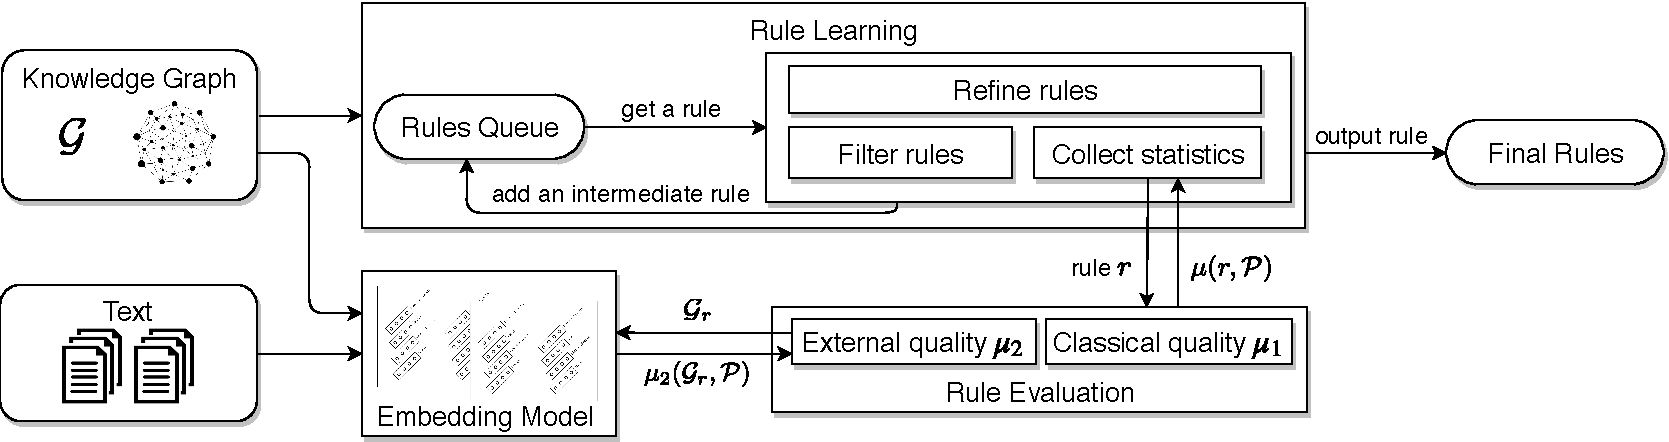
\includegraphics[width=1\textwidth]{figures/system_overview_H.pdf}
\caption{Overview of our system.}
\label{fig:system}
\end{figure}


\subsubsection{Overview.}
%------------------------------------------%
The input of the system are a KG, possibly a text corpus, and a set of user specified parameters that are used to terminate rule construction.
These parameters include an embedding weight $\lambda$, 
a minimum threshold 
for $\mu_1$,  
a minimum rule support $\textit{r-supp}$ 
and other \emph{rule-related} parameters such as a maximum number of positive 
and negative 
atoms allowed in $r$.
The KG and text corpus are used to train the embedding model that in turn is used to construct the probabilistic function $f$.
The rules $r$ are constructed in the iterative fashion, starting from the head, by adding atoms to its body one after another until at least one of the termination criteria (that depend on $f$) is met.
In parallel with the construction of the rule $r$, the quality $\mu(r)$ is computed.
\thi{question from reviewer: how are atoms selected, exactly?}

In Figure~\ref{fig:system} we present a high level architecture of our system, where arrows depict information flow between blocks.
The \emph{Rule Learning} block constructs rules over the input KG, \emph{Rule Evaluation} supplies it with quality scores $\mu$ for rules $r$, using $\cG$ and $f$, where $f$ is computed by the \emph{Embedding Model} block 
from $\cG$ and text.




We now discuss the algorithm behind the \emph{Rule Learning} block
in Figure~\ref{fig:system}. 
Following \cite{amie} we model rules as sequences of atoms, where the first atom is the head of the rule and other atoms are its body. 
The algorithm maintains a priority queue of intermediate rules
(see the \emph{Rules Queue} block in Figure~\ref{fig:system}). 
Initially all possible binary atoms appearing in $\cG$ are added to the queue with empty bodies. 
At each iteration, a single rule is selected from the queue. 
If the rule satisfies the \emph{filtering criteria} 
(see the \emph{Filer rules} block) 
which we define below,
then the system returns it as an output. 
If the rule is not filtered, then it is processed with one of the \emph{refinement operators} 
(see the \emph{Refine rules} block) 
that we define below that expand the rule with one more atom 
and produce new rule candidates, 
which are then pushed into the queue 
(if not being pushed before). 
The iterative process is repeated until the queue is empty. 
All the reported rules will be finally ranked by the decreasing order of the hybrid measure $\mu$, computed in \emph{Collect statistics} block.

In the remainder of the section we discuss refinement operators and filtering criteria.
 


\subsubsection{Refinement operators.}
%------------------------------------------%
We rely on the following three standard refinement operators \cite{amie}
that extend rules:
\begin{enumerate}[label=(\it\roman*)]
\item \textit{add a positive dangling atom}: add a binary positive atom with one fresh variable and another one appearing in the rule, i.e., \emph{shared}.
\item \textit{add a positive instantiated atom}: add a binary positive atom with one argument being a constant and the other one being a shared variable.
\item \textit{add a positive closing atom}: add a binary positive atom with both of its arguments being shared variables.
\end{enumerate}

Additionally, we introduce two more operators to allow negated atoms in rule bodies: 

\begin{enumerate}
\item[\it (iv)] \textit{add an exception instantiated atom}: add a binary negated atom with one of its arguments being a constant, and the other one being a shared variable. 
\item[\it (v)] \textit{add an exception closing atom}: add a binary negated atom to the rule with both of its arguments being shared variables.% 
\end{enumerate}
%
These two operators are only applied to closed rules. 
Moreover, we ensure that the addition of exception atoms to the rule $r:\mi{head(r)\leftarrow body^+(r)}$, 
should result in $r': \mi{head(r)\leftarrow body^+(r), \naf body^-(r)}$, such that 
\[\textit{r-supp}(\mi{head(r)\leftarrow body^+(r), body^-(r)},\cG)=0.\]
Intuitively, we aim at adding exceptions  
that explain the absence of predictions expected to be in the graph rather then their presence. Thus, the introduced exceptions should not affect the rule support, i.e., $\textit{r-supp}(r,\cG) = \textit{r-supp}(r',\cG)$. 

\subsubsection{Filtering criteria.}
%------------------------------------------%
After applying one of the refinement operators to a rule, 
a set of candidate rules is obtained. 
For each candidate rule we first verify that the hybrid measure $\mu$ has increased and discard the rule if it has not. 
Then, we compute its \emph{h-cover}~\cite{amie} and our novel exception confidence measure \emph{e-conf} that are defined as follows:
\begin{align*}
	\textit{h-cover}(r,\cG) & =
		\textit{r-supp}(r,\cG)/
		|\set{h \mid 
				h(head(r,\cG)) \in \G}|,\\
	\textit{e-conf}(r,\cG) & =
		\textit{conf}(r'',\cG),
\end{align*}
where $r'':body^-(r)\leftarrow body^+(r), not\;head(r)$.
If the \emph{h-cover} and \emph{e-conf} are below the user specified threshold, then the rule is discarded.
Intuitively, \emph{h-cover} quantifies the ratio of the known true facts that are implied by the rule.
In contrast, \emph{e-conf} is the conditional probability of the exception given predictions produced by the Horn part of $r$, which helps to disregard insignificant exceptions, i.e., those that explain the absence in $\cG$ of only a small fraction of predictions made by $\mi{head(r)}\leftarrow \mi{body^+(r)}$, as such exceptions likely correspond to noise. 
%
Observe that not all of the filtering criteria are relevant for all rule types. For example, exception confidence is relevant only for non-monotonic rules to ensure the quality of the added exceptions.

Finally, note that by exploiting the embedding feedback, we can now distinguish exceptions from noise. 
Consider the rule stating that married people live together.  This rule can have several possible exceptions, e.g., either one of the spouses is a researcher or he/she works at a company, which has headquarter in the US. Whenever the rule is enriched with an exception, naturally, the support of its body decreases, i.e., the size of $\cG_r$ goes down. 
Relying on our filtering criteria, we aim at 
adding such negated atoms, that the average quality of $\cG_r$ increases, meaning that the introduced negated atoms prevent unlikely predictions.




%!TEX root = ../main.tex

\section{Evaluation}
We have implemented our hybrid rule learning approach in Java within a system prototype RuLES,
and conducted experiments on a Linux machine with 80 cores and 500GB RAM.
In this section we report the results of our experimental evaluation, which focuses on 
\emph{(i)} the benefits of our hybrid embedding-based rule quality measure over traditional rule measures; 
\emph{(ii)} the effectiveness of RuLES against the state-of-art Horn rule learning systems; and 
\emph{(iii)} the quality of non-monotonic rules learned by RuLES compared to existing methods.

\subsection{Experimental Setup}
\label{sec:exper_setup}

\subsubsection{Datasets.}
We performed experiments on the following two real world datasets: 
\begin{itemize}
\item \textit{FB15K}~\cite{Bordes:NIPS2013}: a subset of Freebase with 592K binary facts over 15K entities and 1345 relations
commonly used for evaluating KG embedding models~\cite{DBLP:journals/tkde/WangMWG17}.
\item \textit{Wiki44K}: a dataset with 250K binary facts over 44K entities and 100 relations, which is a subset of 
Wikidata dataset from December 2014
used in~\cite{amie}.
\end{itemize}

In the experiments for each incomplete KG $\G$ we need its \emph{ideal} completion $\G^i$ that would give us a gold standard for evaluating our approach and comparing it to others.
Since obtaining a real life $\G^i$ is hard, we used the KGs FB15K 
and Wiki44K as reference graphs $\cG^i_{appr}$ that approximate $\cG^i$. 
We then constructed $\G$ by randomly selecting $80\%$ of its facts while preserving the distribution of facts over predicates.

\subsubsection{Embedding models.}
We experimented with the three state-of-the-art embedding models:
TransE \cite{Bordes:NIPS2013}, HolE \cite{DBLP:conf/aaai/NickelRP16}, and the text-enhanced SSP \cite{DBLP:conf/aaai/0005HMZ17} model. We reuse the implementation of TransE, HolE\footnote{https://github.com/mnick/scikit-kge}, and SSP\footnote{https://github.com/bookmanhan/Embedding}.
TransE and HolE were trained on $\cG$ and SSP on $\cG$ enriched with 
a textual description for each entity extracted from Wikidata. We compared the
effectiveness of the models and selected for every KG the best one. Apart from SSP, which showed the best performance on both KGs, we also selected HolE for FB15K and TransE for Wiki44K. Note that in this work as a proof of concept we considered some of the most popular embedding models, but conceptually any model (see \cite{DBLP:journals/tkde/WangMWG17} for overview) can be used in our system.


\subsubsection{Evaluation metric.} 
To evaluate the learned rules we use the quality of predictions that they produce 
when applied on $\cG$, i.e., the more correct facts beyond $\cG$ a ruleset produces, the better it is.  
We consider two evaluation settings: \emph{closed world} setting (CW) and \emph{open world} setting (OW). 
In the CW setting, we define the prediction precision of a rule $r$ and a set of rules $R$ as:
\begin{align*}
  pred\_prec_{CW}(r) = \frac{|\cG_r \cap \cG^i_{appr} \setminus \cG|}{|\cG_r \setminus \cG|},
  \quad 
  pred\_prec_{CW}(R) = \frac{\sum\limits_{r\in R} pred\_prec_{CW}(r)}{|R|}.
\end{align*}  
In the OW setting, we also take into account the incompleteness of $\cG^i_{\mi{appr}}$ and  
consider the quality of predictions outside it by performing a random sampling and manually annotating the sampled facts relying on Web resources such as Wikipedia. Thus, we define the OW prediction precision $\mi{pred\_prec_{OW}}$ for a set of rules $R$ as follows:
\[
pred\_prec_{OW}(R) = \frac{|\cG'\cap \cG^i_{\mi{appr}}|+|\cG'\backslash \cG^i_{\mi{appr}}|\times \mi{accuracy(\cG'\backslash \cG^i_{\mi{appr}})}}{|\cG'|}.
\]
where $\cG'=\bigcup_{r\in R}\cG_r\backslash \cG$ is the union of predictions generated by rules in $R$, and $\mi{accuracy(S)}$ is the approximated ratio of true facts inside $S$ computed via manual checking of facts sampled from $S$.
Finally, to evaluate the meaningfulness of exceptions in a rule (i.e., negated atoms) we compute the \textit{revision precision}, which according to~\cite{trantowards} is defined as the ratio of incorrect facts in the difference between predictions produced by the Horn part of a rule and its non-monotonic version over the total number of predictions in this difference (the higher the revision precision, the better the rule exceptions) computed per ruleset. Formally,
\begin{align*}
rev\_prec_{OW}(R) = 1-\frac{|\cG'' \cap \cG^i_{\mi{appr}}|+|\cG''\backslash \cG^i_{\mi{appr}}|\times \mi{accuracy(\cG''\backslash \cG^i_{\mi{appr}})}}{|\cG''|}.
\end{align*}
where $\cG''=\cG_H\backslash \cG_R$ and $H$ is the set of Horn parts of rules in $R$. 
Intuitively, $\G''$ contains facts not predicted by the rules in $R$ but predicted by their Horn versions. 
 
\subsubsection{RuLES configuration.} 
We run RuLES in several configurations where $\mu_1$ is set to either \textit{standard confidence (Conf)} or \textit{PCA confidence (PCA)}, and $\mu_2$ is computed based on either TransE, HolE, or SSP models.
Through the experiments the configurations are named as \textbf{$\mu_1$-$\mu_2$} (e.g. Conf-HolE).


\subsection{Embedding-Based Hybrid Quality Function}
\captionsetup[subfigure]{textfont=scriptsize}
 \begin{figure}[t]
     \centering
      %Gad: to unify legend and save space
     \subfloat{{
\includegraphics[width=0.6\textwidth]{figures/new_exp1/legend-crop.pdf} }}\\[-1ex]
     \setcounter{subfigure}{0}
     \subfloat[Conf-HolE on FB15K]{{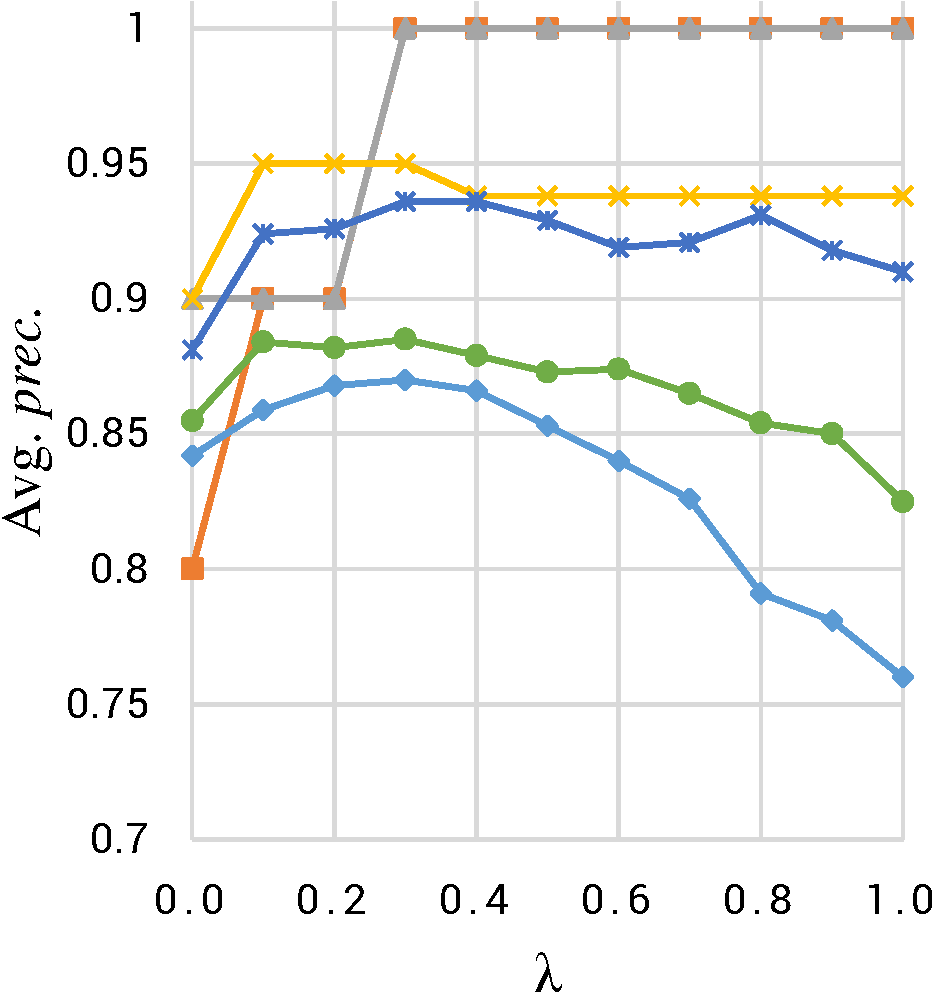
\includegraphics[width=0.3\textwidth]{figures/new_exp1/fb15k_hole_conf-crop.pdf} }\label{fig:fb-HoLE-Conf}}
     \subfloat[Conf-SSP on FB15K]{{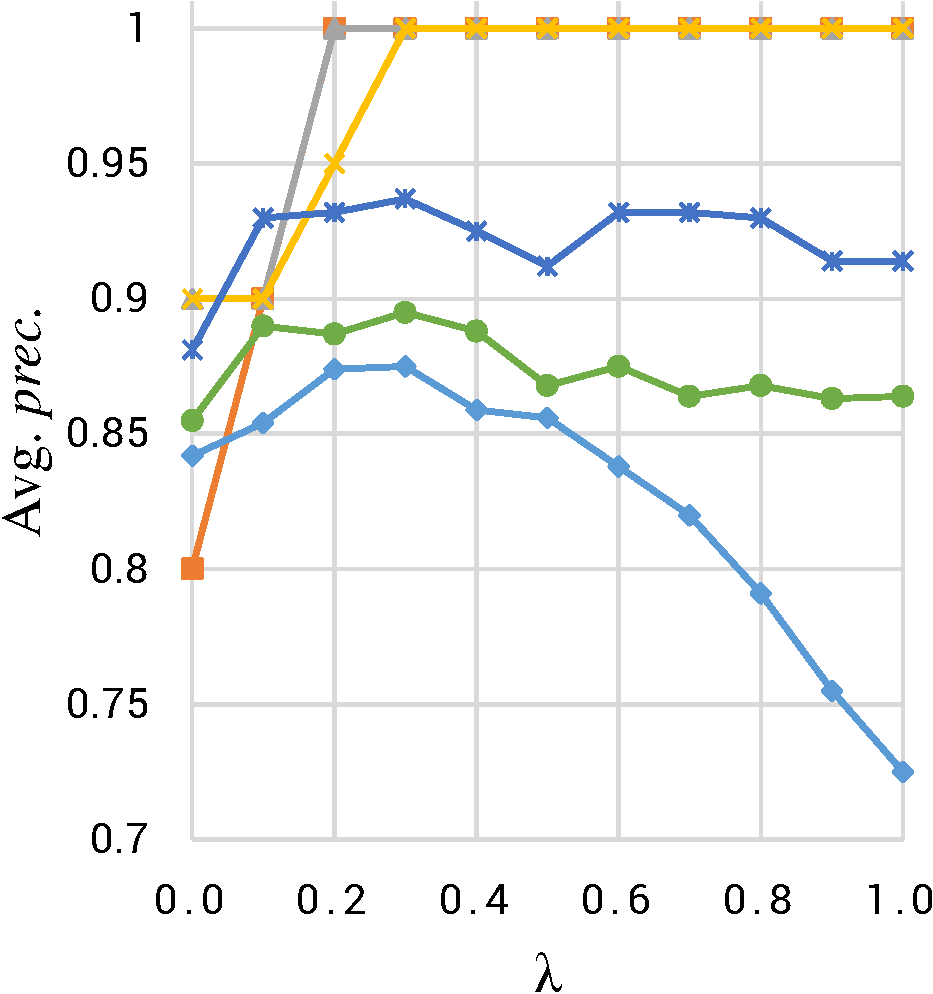
\includegraphics[width=0.3\textwidth]{figures/new_exp1/fb15k_ssp_conf-crop.pdf} \label{fig:fb-SSP-Conf}}}
     %\subfloat[RulES-H-PCA on FB15K]{{\includegraphics[width=0.3\textwidth]{figures/fb15k_hole_pca-crop.pdf} }}
    \subfloat[PCA-SSP on FB15K]{{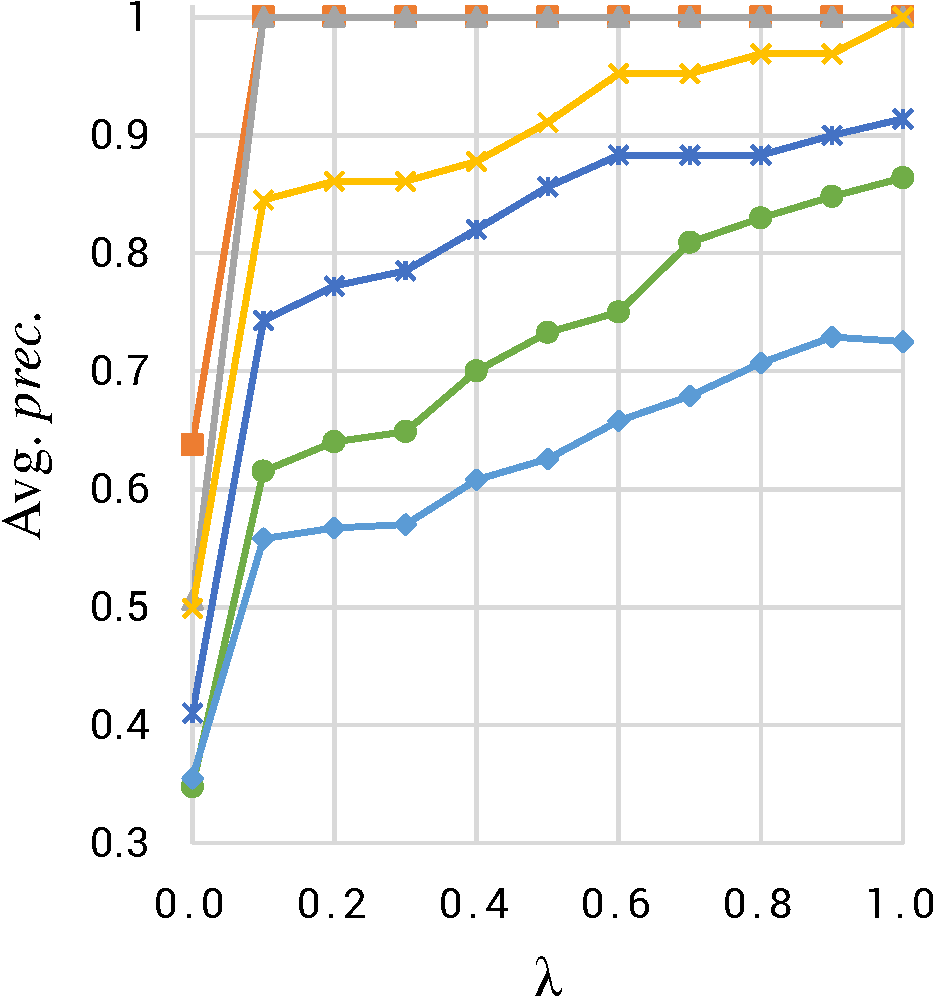
\includegraphics[width=0.3\textwidth]{figures/new_exp1/fb15k_ssp_pca-crop.pdf} }\label{fig:fb-SSP-PCA}} \\   
    
    \subfloat[Conf-TransE on Wiki44K]{{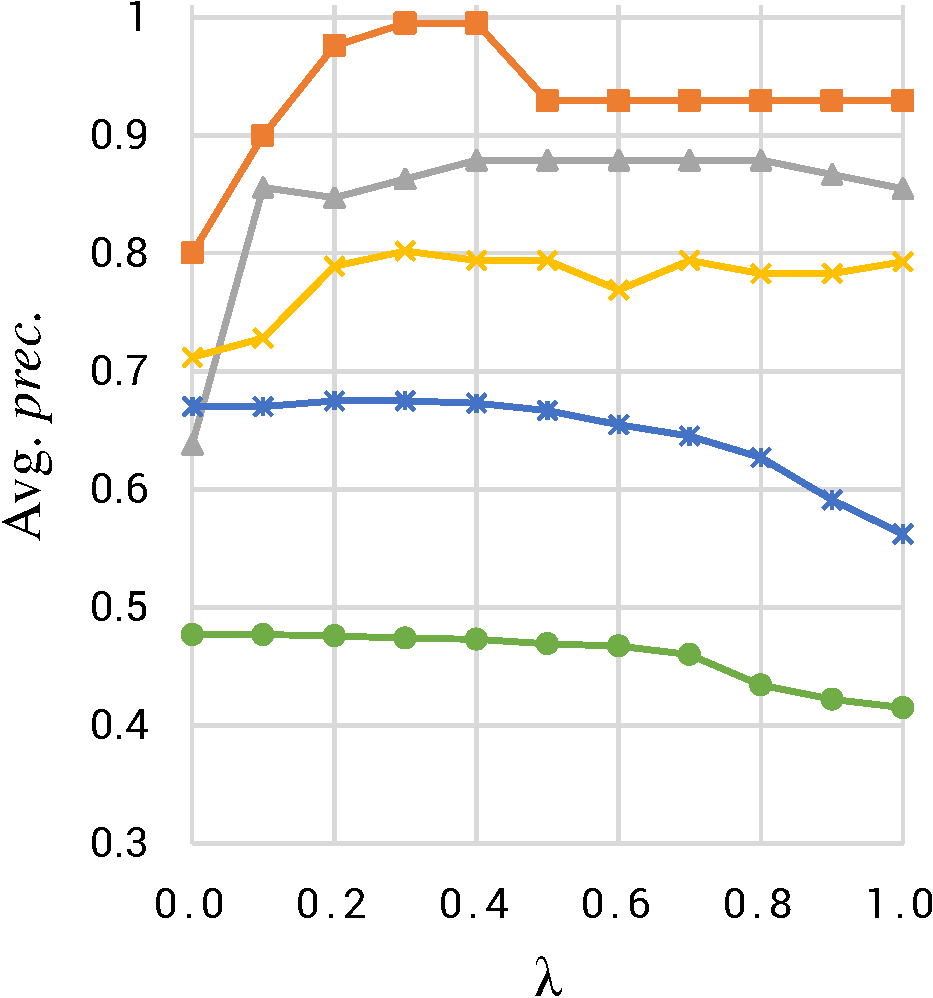
\includegraphics[width=0.3\textwidth]{figures/new_exp1/wiki44k_transe_conf-crop.pdf} }\label{fig:wi-TransE-Conf}}
    \subfloat[Conf-SSP on Wiki44K]{{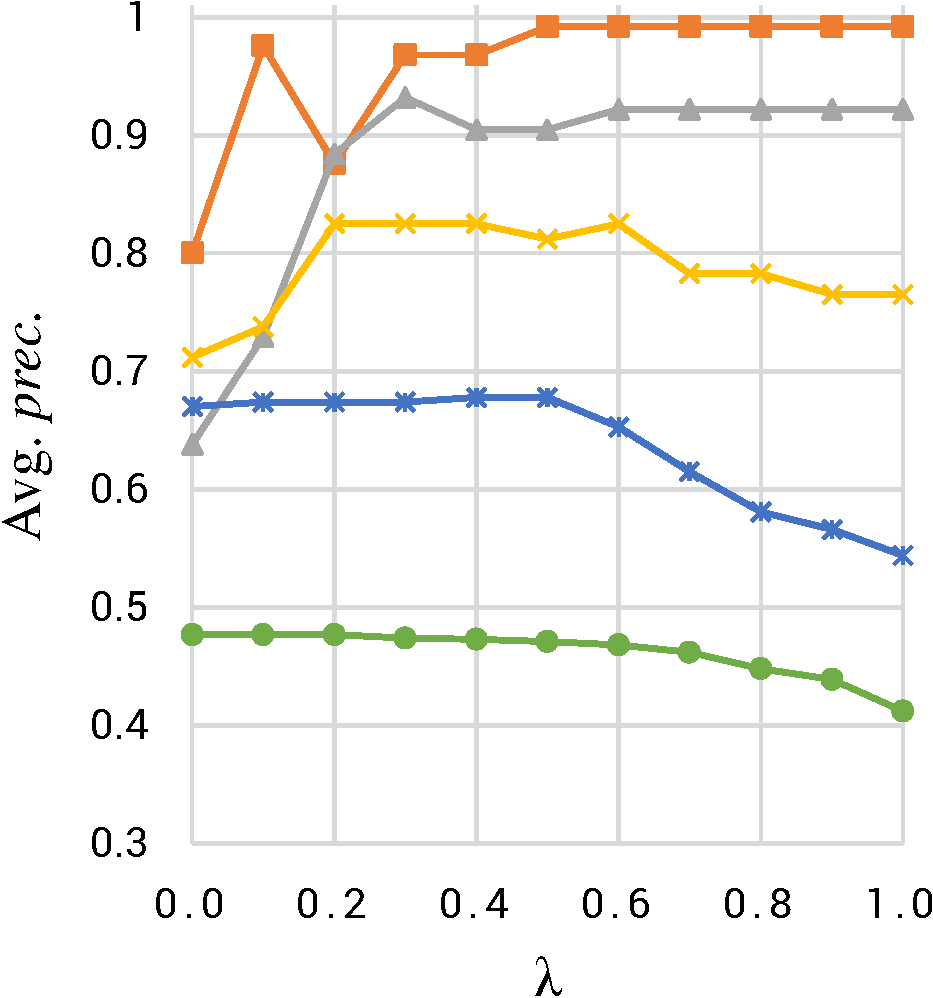
\includegraphics[width=0.3\textwidth]{figures/new_exp1/wiki44k_ssp_conf-crop.pdf} }\label{fig:wi-SSP-Conf}}
     %\subfloat[RulES-H-PCA on Wiki44K]{{\includegraphics[width=0.3\textwidth]{figures/wiki44k_transe_pca-crop.pdf} }}
     \subfloat[PCA-SSP on Wiki44K]{{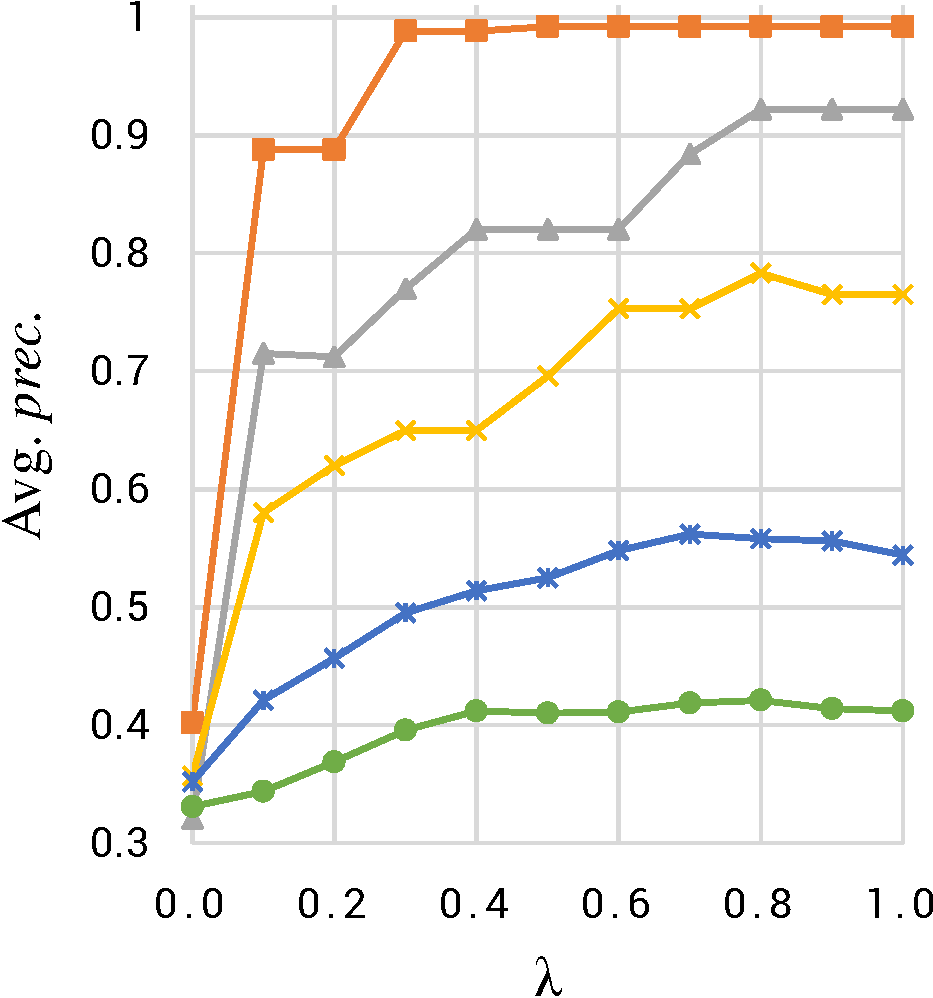
\includegraphics[width=0.3\textwidth]{figures/new_exp1/wiki44k_ssp_pca-crop.pdf} }\label{fig:wi-SSP-PCA}} \\  
    
     \caption{$pred\_prec_{CW}$ of the \textit{top-k} rules with various \textit{embedding weights}.}
     \label{fig:diff_lambda}
 \end{figure}
%\captionsetup[subfigure]{labelformat=empty}
%\begin{figure}[t]
%    \centering    
%    % \vspace*{-3mm}
%    \subfloat{{
\includegraphics[width=0.5\textwidth]{figures/new_exp1/legend-crop.pdf} }}\\[-2ex]
%    \subfloat[FB15K(conf + HolE)]{{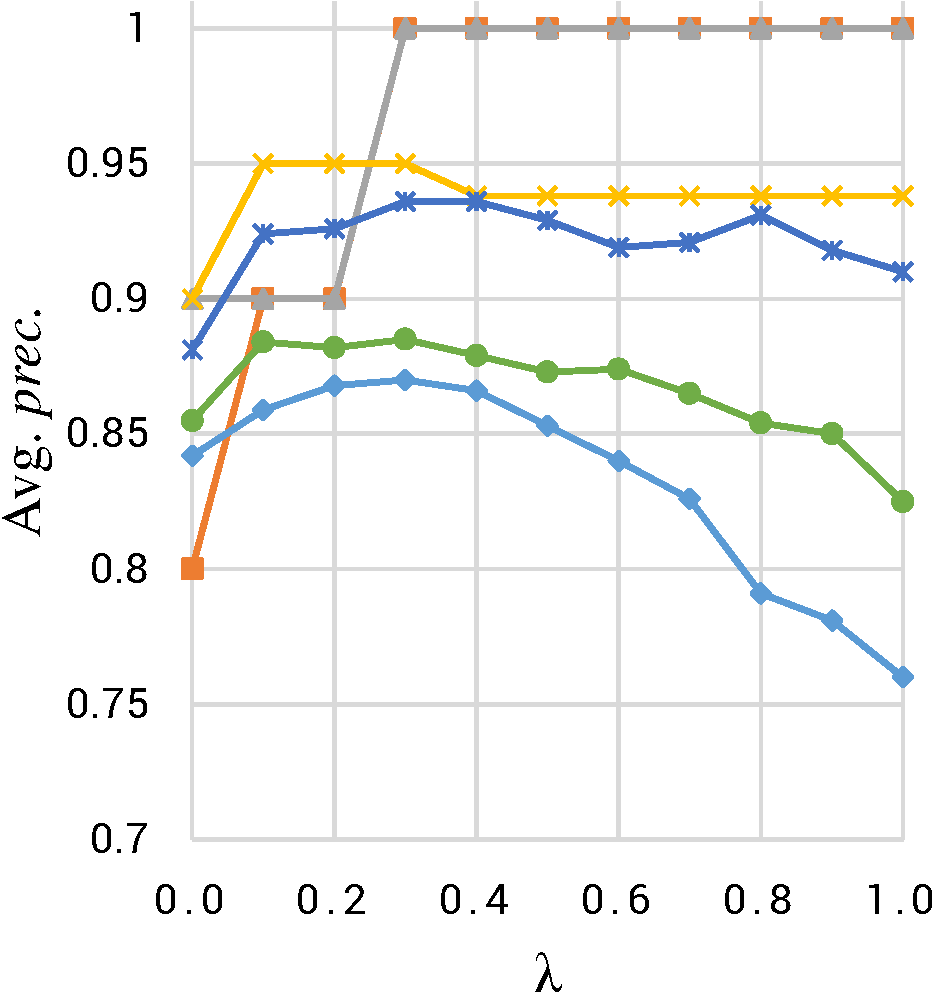
\includegraphics[width=0.33\textwidth]{figures/new_exp1/fb15k_hole_conf-crop.pdf} }}
%    \subfloat[FB15K(conf + SSP)]{{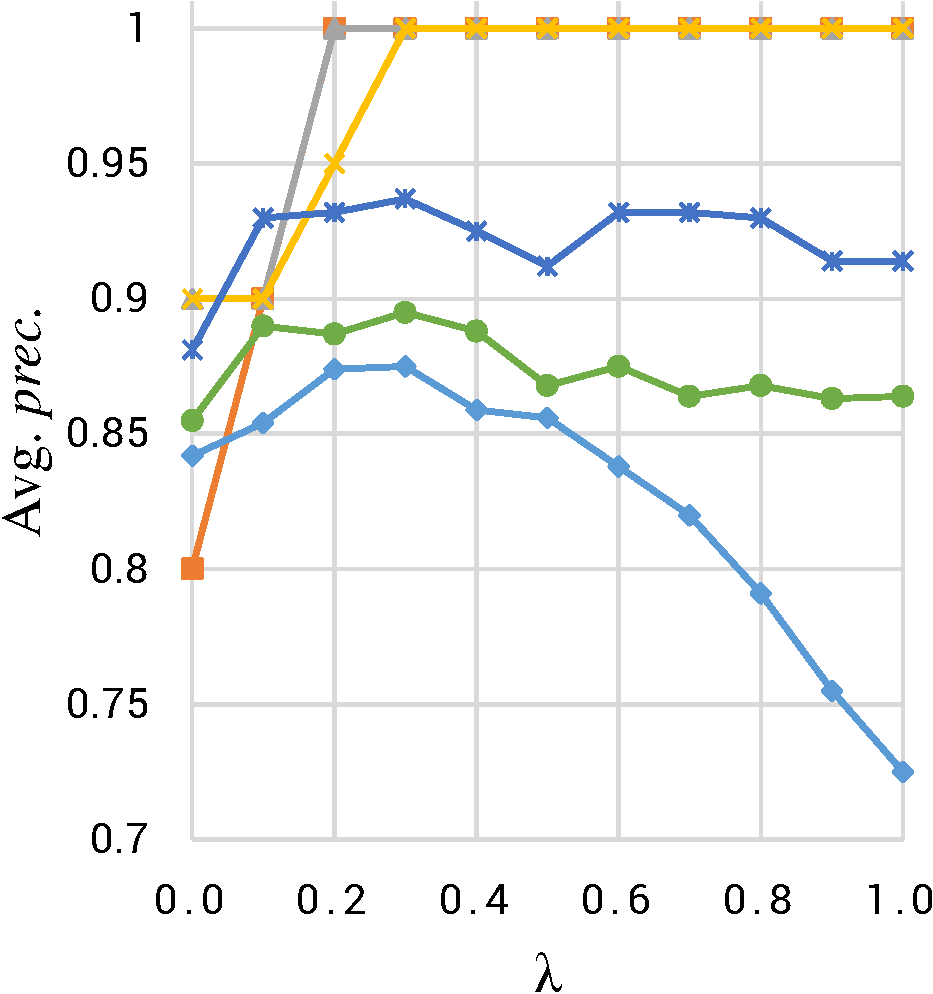
\includegraphics[width=0.33\textwidth]{figures/new_exp1/fb15k_ssp_conf-crop.pdf} }}
%    % \subfloat[PCA Confidence + HolE]{{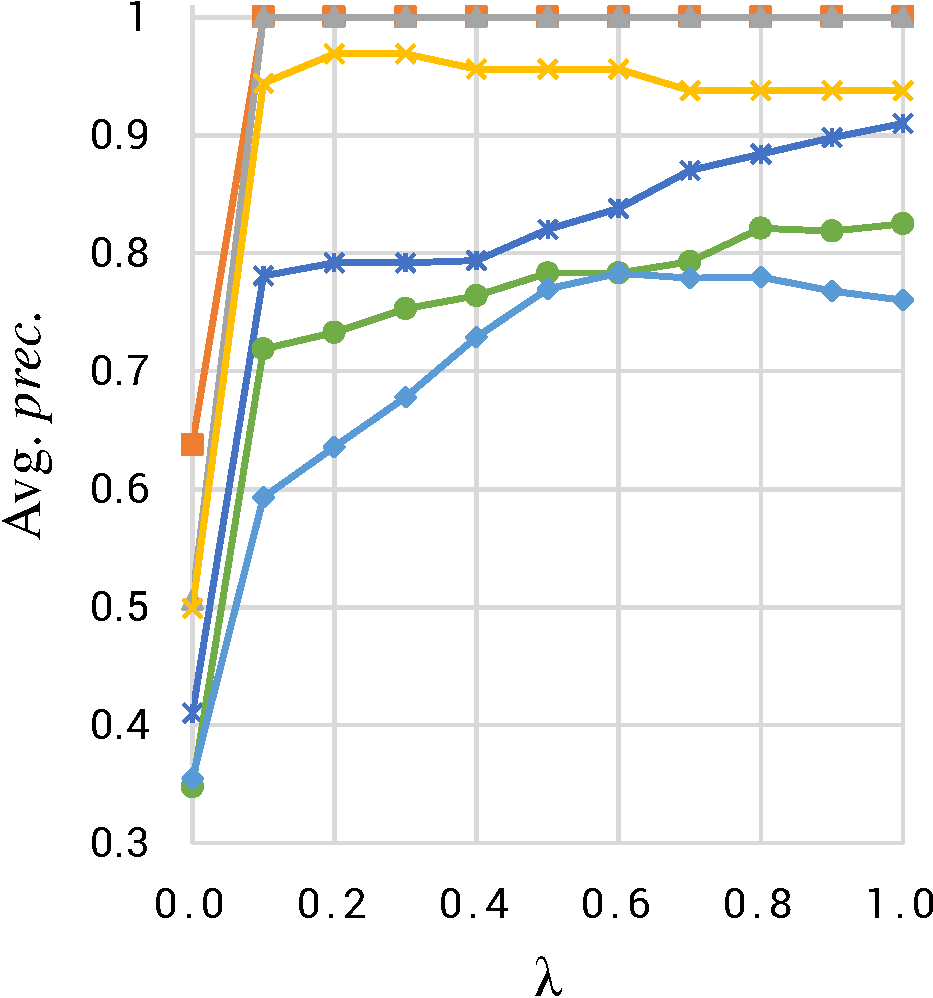
\includegraphics[width=0.5\textwidth]{figures/new_exp1/fb15k_hole_pca-crop.pdf} }}
%    \subfloat[FB15K(pcaconf + SSP)]{{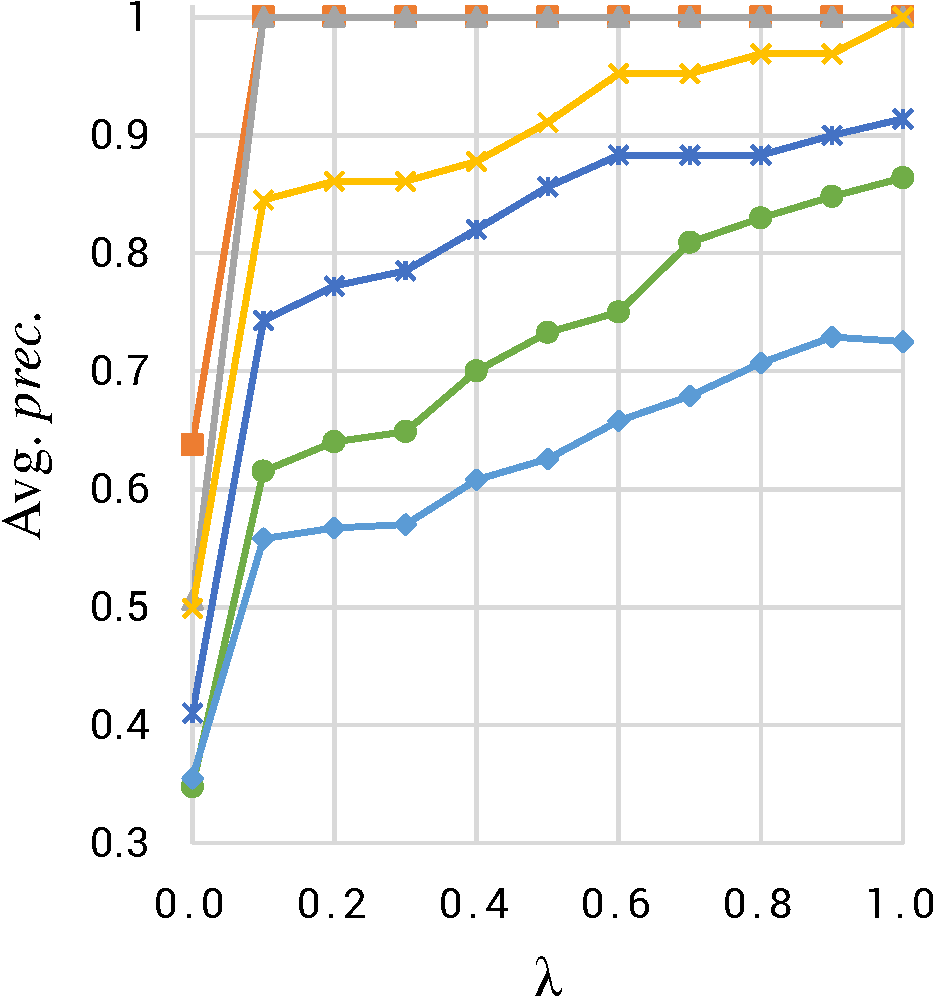
\includegraphics[width=0.33\textwidth]{figures/new_exp1/fb15k_ssp_pca-crop.pdf} }}\\
%    \subfloat[Wiki44K(conf + TransE)]{{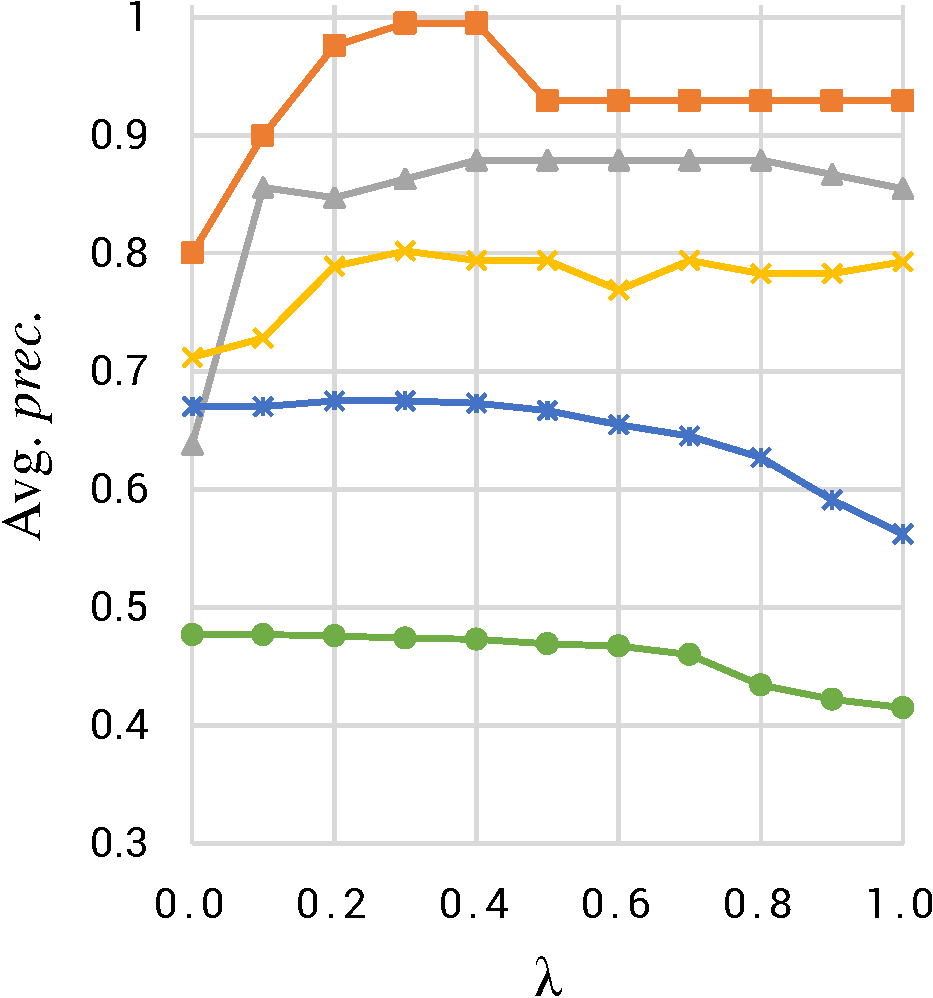
\includegraphics[width=0.33\textwidth]{figures/new_exp1/wiki44k_transe_conf-crop.pdf} }}
%    \subfloat[Wiki44K(conf + SSP)]{{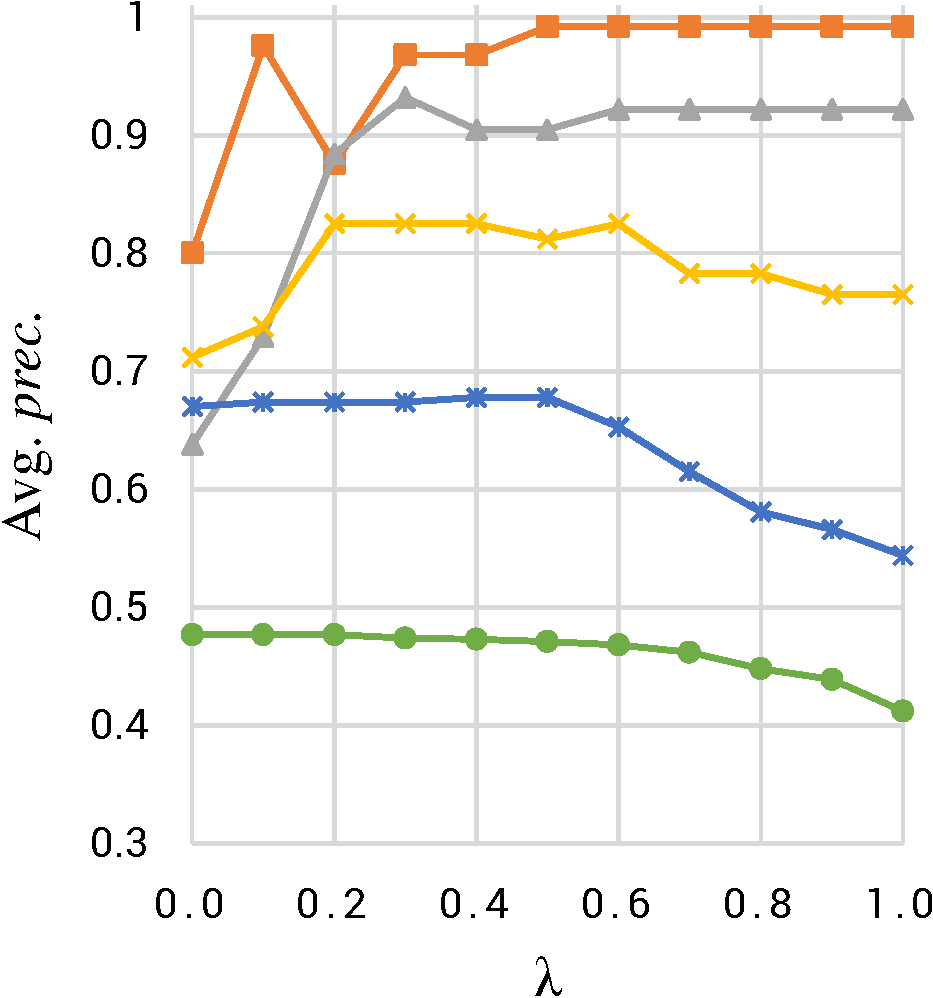
\includegraphics[width=0.33\textwidth]{figures/new_exp1/wiki44k_ssp_conf-crop.pdf} }}
%    % \subfloat[PCA Confidence + TransE]{{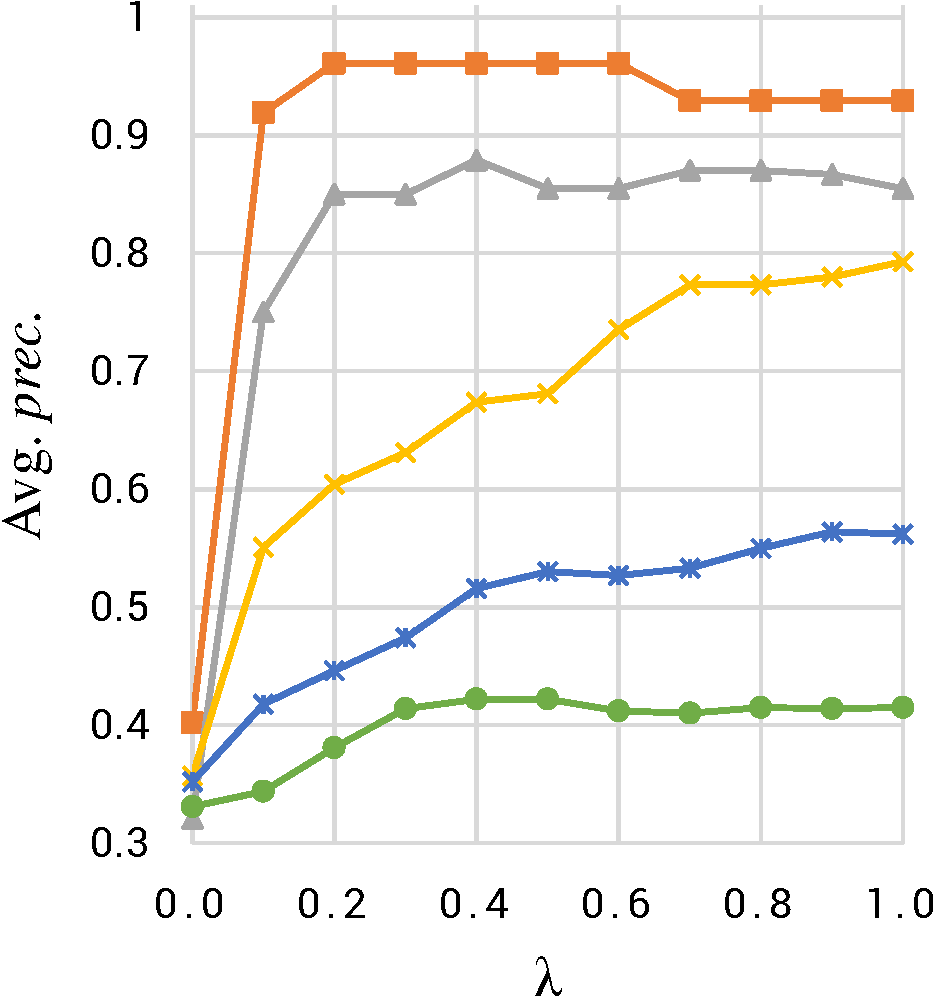
\includegraphics[width=0.5\textwidth]{figures/new_exp1/wiki44k_transe_pca-crop.pdf} }}
%    \subfloat[Wiki44K(pcaconf + SSP)]{{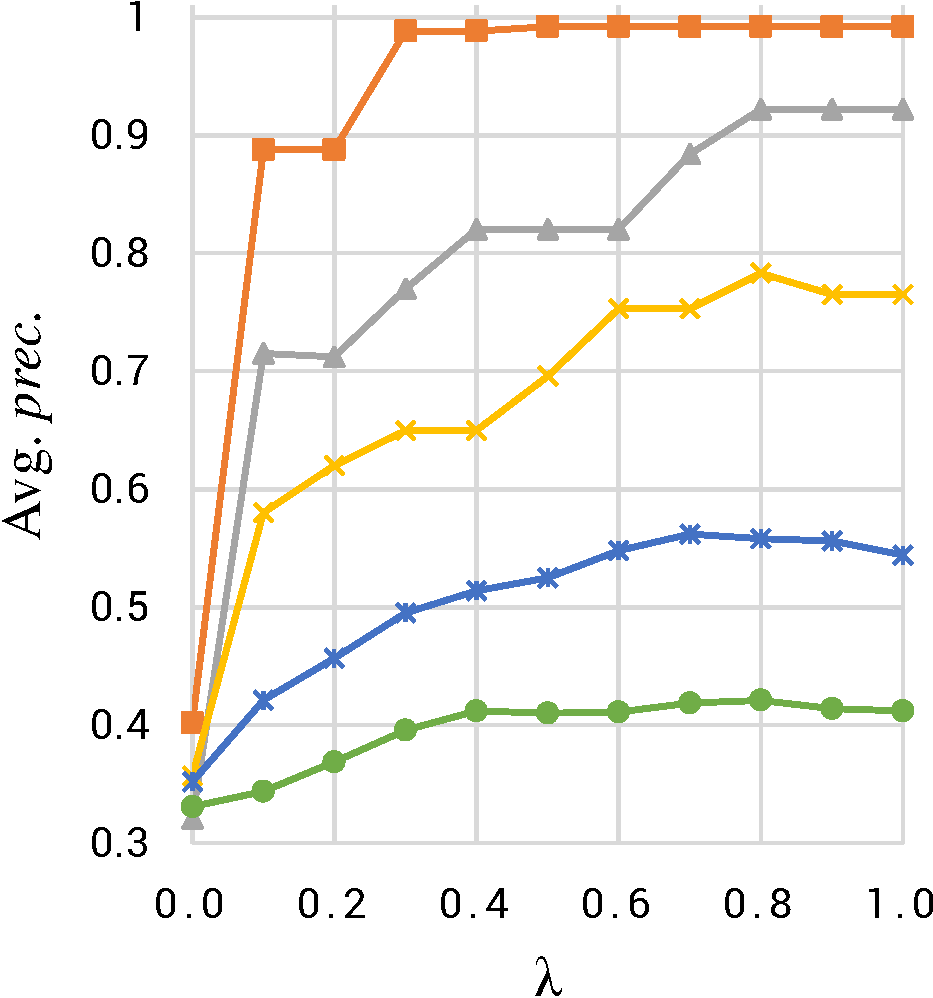
\includegraphics[width=0.33\textwidth]{figures/new_exp1/wiki44k_ssp_pca-crop.pdf} }}\\
%    
%    \caption{Avg. \textit{predictions precision} of the top rules with various \textit{embedding weights} \gad{figures labels should be updated and height should be reduced }}
%    \label{fig:fb15k_and_wiki44k}
%\end{figure}
In this experiment we study the effect of using our hybrid embedding-based 
rule measure $\mu$ from Equation~\ref{eq:hm} on the 
rule ranking compared to traditional measures \add{and embedding models independently. }
We do it by first 
learning rules of the form $r:\;h(X,Z) \leftarrow p(X,Y), q(Y,Z)$ from $\cG$ where $\mi{\textit{r-supp}(r,\cG)\geq 10}$, $\mi{conf(r,\cG)\in [0.1,1)}$ and $\mi{\textit{h-cover}(r,\cG)\geq 0.01}$. 
Then, we rank these rules using Equation~\ref{eq:hm} with $\lambda\in \{0, 0.1, 0.2, \dotsc, 1\}$, $\mu_1\in \{\mi{conf,conf_{pca}}\}$ and with $\mu_2$ that is computed by relying on TransE, HolE and SSP.
\dl{Note that $\lambda=0$ corresponds to the standard rule measure $\mu_1$ alone.}
\add{Note that $\lambda=0$ simulates learning rules using the standard measure $\mu_1$ similar to~\cite{amie}, while $\lambda=1$ corresponds to ranking rules solely based on the predictions of the embedding models. Configuring $\lambda$ indirectly allows us to compare our hybrid measure to both traditional measures and quality of embedding models.}

Figure~\ref{fig:diff_lambda} shows the 
average prediction precision $pred\_prec_{CW}$ of the \textit{top-k} rules ranked using our measure $\mu$ for different embedding weights $\lambda$ (\textit{x-axis}). 
In particular, in Figures~\ref{fig:fb-HoLE-Conf},~\ref{fig:fb-SSP-Conf},~\ref{fig:wi-TransE-Conf}, and~\ref{fig:wi-SSP-Conf} 
we observe that combining confidence with any 
embedding model increases the average prediction precision for $0\leq \lambda\leq 0.3$. 
Moreover, we observe the decrease of prediction precision for $0.4 \leq \lambda\leq 1$ and \textit{top-k} rules learned from FB15K when $k\geq 20$ and from Wiki44K when $k\geq 10$. 
This 
shows that the combination of $\mu_1$ and $\mu_2$ gives noticeable positive effect 
on the prediction results. \add{Ranking using hybrid measure with $\lambda$ around 0.3 achieves better results than both the traditional rule learning and embedding models.} On the other hand, for $\mu_1=\mi{conf_{pca}}$ the precision increases significantly when combined with embedding models and only decreases slightly 
for $\lambda=1$ (Figures~\ref{fig:fb-SSP-PCA},\ref{fig:wi-SSP-PCA}). 
Utilizing $\mi{conf_{pca}}$ instead of $\mi{conf}$ as $\mu_1$ in our hybrid measure is less effective, since 
our training data $\cG$ is randomly sampled 
breaking the 
partial completeness assumption adopted by the PCA confidence. 

\begin{table}[t]
\scriptsize
%\tiny
\centering
\begin{tabular}{c |r r r r |r r r r} 
 \multirow{3}{*}{\textbf{\textit{top-k}}} & \multicolumn{4}{c}{\textbf{FB15K}} & \multicolumn{4}{|c}{\textbf{Wiki44K}} \\
 \cmidrule{2-9}
 & \textbf{{~~}Conf}&  \textbf{{~~~~~~~~}PCA} & \textbf{Conf-HolE}& \textbf{Conf-SSP} &  \textbf{{~~}Conf}&  \textbf{{~~~~~~~~}PCA} & \textbf{Conf-TransE}& \textbf{Conf-SSP}\\
  & {\scriptsize($\lambda=0$)}  & {\scriptsize($\lambda=0$)} & {\scriptsize($\lambda=0.3$)} & {\scriptsize($\lambda=0.3$)} & {\scriptsize($\lambda=0$)} & {\scriptsize($\lambda=0$)} &{\scriptsize($\lambda=0.3$)} & {\scriptsize($\lambda=0.3$)}\\
 \midrule
 \textbf{5} & 0.800 & 0.638 & \textbf{1.000} & \textbf{1.000} & 0.800 & 0.402 & \textbf{0.995} & 0.968\\
\textbf{10} & 0.900 & 0.506 & \textbf{1.000} & \textbf{1.000} & 0.638 & 0.321 & 0.863 & \textbf{0.932} \\
\textbf{20} & 0.900 & 0.499 & 0.950 & \textbf{1.000} & 0.712 & 0.357 & 0.802 & \textbf{0.825}\\
\textbf{50} & 0.881 & 0.410 & 0.936 & \textbf{0.937} & 0.670 & 0.352 & \textbf{0.675} & 0.674 \\
\textbf{100} & 0.855 & 0.348 & 0.885 & \textbf{0.895} & \textbf{0.477} & 0.331 & 0.474 & 0.474\\
\textbf{200} & 0.842 & 0.355 & 0.870 & \textbf{0.875} & -- & -- & -- & -- \\
 \bottomrule
\end{tabular}
\caption{$pred\_prec_{CW}$ of the \textit{top-k} rules learned using different measures.}
\label{table:avg_quality}
\vspace*{-3mm}
\end{table}


Table~\ref{table:avg_quality} compactly summarizes the average prediction precision of \textit{top-k} rules ranked by
the standard rule measures and our $\mu$ for the best value of $\lambda=0.3$ and highlights the effect of using the better embedding model (text-enhanced vs standard).
We observe that the accuracy of a utilized embedding model is naturally propagated to the accuracy of the rules that we obtain using our hybrid ranking measure $\mu$. This demonstrates that the use of a better embedding model positively effects 
the quality of learned rules. 


\subsection{Horn Rule Learning}
\label{sec:RuLES_vs_AMIE}

\begin{table}[t]
\scriptsize
\centering
\begin{tabular}{c|r r|r r|r r|r r|r r|r r}

 \multirow{3}{*}{\textbf{\textit{top-k}}}&\multicolumn{6}{|c}{\textbf{FB15K}} & \multicolumn{6}{|c}{\textbf{Wiki44K}}\\
 \cmidrule{2-13}&\multicolumn{2}{|c}{\textbf{AMIE-PCA}}&\multicolumn{2}{|c|}{\textbf{AMIE-Conf}}&\multicolumn{2}{|c}{\textbf{RuLES}}&\multicolumn{2}{|c}{\textbf{AMIE-PCA}}&\multicolumn{2}{|c}{\textbf{AMIE-Conf}}&\multicolumn{2}{|c}{\textbf{RuLES}} \\
 & \textit{Facts} & \textit{Prec.} & \textit{Facts} & \textit{Prec.} & \textit{Facts} & \textit{Prec.} &\textit{Facts} & \textit{Prec.} &\textit{Facts} & \textit{Prec.} &\textit{Facts} & \textit{Prec.} \\
 \midrule
 \textbf{20} & 1029 & 0.28 & 82 & 0.63 & 44 & 1.00 & 185 & 0.73 & 91 & 0.95 & 3291 & 0.98\\
 \textbf{50} & 1716 & 0.43 & 190 & 0.74 & 186 & 0.92 & 47099 & 0.10 & 3594 & 0.95 & 6154 & 0.88 \\
\textbf{100} & 3085 & 0.65 & 255 & 0.78 & 539 & 0.80 & 56831 & 0.20 & 13870 & 0.83 & 13253 & 0.82 \\
\textbf{200} & 10586 & 0.62 & 1210 & 0.83 & 1205 & 0.88 & 82288 & 0.39 & 19538 & 0.72 & 20408 & 0.73 \\
\textbf{500} & 40050 & 0.51 & 2702 & 0.75 & 7124 & 0.95 & 219264 & 0.35 & 124836 & 0.23 & 128256 & 0.48 \\
 \bottomrule
\end{tabular}
\caption{$pred\_prec_{OW}$ of the \textit{top-k} rules generated by RuLES and AMIE.}
\label{table:amie_vs_RuLES}
\vspace*{-3mm}
\end{table}

\begin{table}[t]
\scriptsize
\centering
\begin{tabular}{c|r r|r r}

 \multirow{2}{*}{}&\multicolumn{2}{c}{\textbf{Family-NeuralLP}}&\multicolumn{2}{|c}{\textbf{Family-Conf-TransE}}\\
\textbf{\emph{top-k}}& \textit{Facts} & \textit{Prec.} & \textit{Facts} & \textit{Prec.} \\
 \midrule
\textbf{10} & 3709 & 0.72 & 4201 & 0.68 \\
\textbf{20} & 8821 & 0.53 & 6957 & 0.72 \\
\textbf{30} & 11337 & 0.49 & 9368 & 0.71 \\
\textbf{40} & 14662 & 0.46 & 11502 & 0.72 \\
\textbf{50} & 18768 & 0.40 & 14547 & 0.62 \\
 \bottomrule
\end{tabular}
\caption{$pred\_prec_{OW}$ of the \textit{top-k} rules generated by NeuralLP and RuLES.}
\label{table:neurallp_vs_rules}
%\thi{This is added to compare NeuralLP and RuLES}
\vspace*{-3mm}
\end{table}


In this experiment, we compare RuLES under Conf-SSP configuration (with embedding weight $\lambda = 0.3$) with the state-of-art Horn rule learning system AMIE. We used the default AMIE-PCA configuration with $\mi{conf_{pca}}$ and 
AMIE-Conf with $\mi{conf}$ measures respectively. For a fair comparison, we set the two configurations of AMIE and our system  to generate rules with at most three positive atoms and filtered them based on minimum confidence of $0.1$, head coverage of $0.01$ and rule support of $10$ in case of FB15K and $2$ in case of Wiki44K. We then filtered out all rules with $\mi{conf(r,\cG) = 1}$, as they 
do not produce any predictions.

Table~\ref{table:amie_vs_RuLES} shows the number of facts (see the \textit{Facts} column) predicted by 
the set $R$ of \textit{top-k} rules 
in the described settings 
and their prediction precision $pred\_prec_{OW}(R)$ (see the \textit{Prec.} column). 
The size of the random sample 
outside $\cG^i_{appr}$ is 20. 
We can observe that on FB15K, RuLES consistently outperforms both AMIE configurations. The \textit{top-20} rules have the highest precision difference (outperforming AMIE-PCA and AMIE-Conf by $72\%$ and $37\%$ respectively).
This is explained by the fact that the hybrid embedding quality penalizes rules with higher number of false predictions. 
For Wiki44K, RuLES is capable of achieving better precision in most of the cases. 
Notably, for the \textit{top-20} rules RuLES predicted significantly more facts then competitors yet with a high precision. 

In table~\ref{table:neurallp_vs_rules}, we compare RuLES with the recently developed NeuralLP system~\cite{DBLP:conf/nips/YangYC17}. For this we 
utilized the Family dataset used by NeuralLP 
with 28K facts over 3K entities and 12 relations. 
Starting from the \textit{top-20} rules RuLES is capable of achieving significantly better precision. For the \textit{top-10} rules the precision of NeuralLP is slightly better, but RuLES predicts many more facts.


\subsection{RuLES for Exception-Aware Rule Learning}
%----------------------------------------------------------------%
In this experiment, we aim at evaluating the effectiveness of RuLES 
for learning exception-aware rules.
First, consider in Table~\ref{figure:examples} examples of such rules learned by RuLES over Wiki44K dataset. 
 The first rule $r^1$ says that a person is a citizen of the country where his alma mater is located, unless it is a research institution, 
since most 
researchers in universities are foreigners. The second rule $r^2$ states that the scriptwriter of some artistic work is also the scriptwriter of its sequel unless it is a TV series, which actually reflects the common practice of having several screenwriters for different seasons. Additionally, $r^3$ encodes that someone belonged to a 
noble family if his/her 
spouse is also from the same noble family, excluding the Chinese dynasties. 

To quantify the quality of RuLES in learning non-monotonic rules, we compare the Conf-SSP configuration of RuLES (with embedding weight $\lambda = 0.3$) with RUMIS~\cite{trantowards}, which is a revision-based 
non-monotonic rule 
learning system, which 
extracts rules 
of the form  
$\mi{r:\;h(X,Z) \leftarrow p(X,Y), q(Y,Z), not\; E}$, where $E$ is either $e(X,Z)$ or 
$e(X)$.
For a fair comparison we restricted RuLES to learn rules of the same form.   
We configured both systems 
setting the minimum rule support threshold to 
$10$ and exception confidence for RuLES to $0.05$. 
To enable the systems to 
learn rules with exceptions of the form 
$e(X)$, we enriched 
our KGs with \textit{types} 
from original Freebase and Wikidata KGs. 

%!TEX root = ../main.tex


\begin{table}[t]
\centering
\footnotesize
\begin{tabular}{|cl|}
	\hline
	%$r_1:$ & $has\_family(X, Y) \leftarrow has\_child(Z, X), has\_family(Z, Y), \textbf{not}\ has\_mother(X, Z).$\\
$r^1{:}$ & $\mi{nationality(X{,}\, Y)}\, {\leftarrow}\, \mi{graduated\_from(X{,}\, Z)}{,}\, \mi{in\_country(Z{,}\, Y)},
	\textbf{not}\ \mi{research\_uni(Z)}$\\
$r^2{:}$ & $\mi{scriptwriter\_of}(X{,}\, Y)\, {\leftarrow}\, \mi{preceded\_by(X{,}\, Z)}{,}\, \mi{scriptwriter\_of(Z{,}\, Y)},
\textbf{not}\ \mi{tv\_series(Z)}$\\
$r^3{:}$ &$\mi{noble\_family(X{,}\, Y)}\, {\leftarrow}\, \mi{ spouse(X{,}\, Z)}{,}\, \mi{noble\_family(Z{,}\, Y)}{,}\,  \textbf{not}\ \mi{ chinese\_dynasties(Y)}$\\
%$r_3:$ &$\mi{sister(X, Y)} \leftarrow \mi{sister(Y, X)}, \textbf{not}\ \mi{brother(X, Y)}$\\

	\hline
\end{tabular}
\caption{Example rules with exception generated by RuLES.}
\vspace*{-3mm}
\label{figure:examples}
\end{table}

%!TEX root = ../main.tex

% \begin{table}[t]
% \centering
% \begin{tabular}{|r|r r|r r|r r|r r|}
%  \hline
%  \multirow{3}{*}{$top-k$}&\multicolumn{4}{|c|}{FB15K} & \multicolumn{4}{|c|}{WIKI44K}\\
%  \cline{2-9}&\multicolumn{2}{|c|}{RUMIS}&\multicolumn{2}{|c|}{RuLES}&\multicolumn{2}{|c|}{RUMIS}&\multicolumn{2}{|c|}{RuLES} \\
%  & $Avg.scr.$ & $Avg.inc.$ & $Avg.scr.$ & $Avg.inc.$& $Avg.scr.$ & $Avg.inc.$& $Avg.scr.$ & $Avg.inc.$ \\
%  \hline
%  20 & 0.791 & 0.024 & 1.000 & 0.047 & 0.743 & 0.067 & 0.803 & 0.024 \\
%  50 & 0.826 & 0.015 & 1.000 & 0.045 & 0.609 & 0.054 & 0.701 & 0.026 \\
% 100 & 0.859 & 0.026 & 0.990 & 0.047 & 0.417 & 0.033 & 0.539 & 0.011 \\
% 200 & 0.848 & 0.034 & 0.977 & 0.065 & 0.253 & 0.022 & 0.339 & 0.017 \\
% 500 & 0.745 & 0.043 & 0.958 & 0.079 & -- & -- & -- & -- \\
% \hline
% \end{tabular}
% \caption{Average prediction score of some top non-monotonic rules from RuLES vs RUMIS.}
% \label{table:exception_prediction_result}
% \vspace*{-3mm}
% \end{table}

%\begin{table}[t]
%\centering
%\begin{tabular}{|c|r r|r r|r r|r r|}
% \hline
% \multirow{3}{*}{\textbf{\textit{top-k}}}&\multicolumn{4}{|c|}{\textbf{FB15K}} & \multicolumn{4}{|c|}{\textbf{Wiki44K}}\\
% \cline{2-9}&\multicolumn{2}{|c|}{\textbf{RUMIS}}&\multicolumn{2}{|c|}{\textbf{RuLES}}&\multicolumn{2}{|c|}{\textbf{RUMIS}}&\multicolumn{2}{|c|}{\textbf{RuLES}} \\
% & $Facts$ & $Prec.$ & $Facts$ & $Prec.$& $Facts$ & $Prec.$& $Facts$ & $Prec.$ \\
% \hline
%\textbf{20} & 672 & 0.95 & 34 & 0.97 & 5844 & 0.93 & 5640 & 0.93 \\
%\textbf{50} & 1797 & 0.94 & 158 & 0.99 & 8585 & 0.83 & 13333 & 0.84 \\
%\textbf{100} & 2672 & 0.94 & 434 & 0.99 & 21081 & 0.76 & 25265 & 0.81 \\
%\textbf{200} & 4103 & 0.87 & 1155 & 0.96 & 50957 & 0.51 & 43677 & 0.67 \\
%\textbf{500} & 13439 & 0.76 & 5466 & 0.90 & -- & -- & -- & -- \\
%\hline
%\end{tabular}
%\caption{$pred\_prec_{OW}$ of the \textit{top-k} rules learned by RUMIS and RuLES.}
%\label{table:exception_prediction_result}
%\vspace*{-3mm}
%\end{table}

\begin{table}[t]
\scriptsize
\centering
\begin{tabular}{r | r r| r r | r r |r r}
 & \multicolumn{4}{c}{\textbf{FB15K}} & \multicolumn{4}{|c}{\textbf{Wiki44K}} \\
 \cmidrule{2-9}&\multicolumn{2}{c}{\textbf{RUMIS}}&\multicolumn{2}{|c}{\textbf{RuLES}}&\multicolumn{2}{|c}{\textbf{RUMIS}}&\multicolumn{2}{|c}{\textbf{RuLES}} \\
\textbf{\textit{top-k}} & \emph{Facts} & \emph{Prec.} & \emph{Facts} & \emph{Prec.} & \emph{Facts} & \emph{Prec.}& \emph{Facts} & \emph{Prec.} \\
 \midrule
\textbf{20} & 672 & 0.95 & 34 & 0.97 & 5844 & 0.93 & 5640 & 0.93 \\
\textbf{50} & 1797 & 0.94 & 158 & 0.99 & 8585 & 0.83 & 13333 & 0.84 \\
\textbf{100} & 2672 & 0.94 & 434 & 0.99 & 21081 & 0.76 & 25265 & 0.81 \\
\textbf{200} & 4103 & 0.87 & 1155 & 0.96 & 50957 & 0.51 & 43677 & 0.67 \\
\textbf{500} & 13439 & 0.76 & 5466 & 0.90 & -- & -- & -- & -- \\
\bottomrule
\end{tabular}
%
\qquad
%
\begin{tabular}{r | r r| r r | r r |r r}
 & \multicolumn{4}{c}{\textbf{FB15K}} & \multicolumn{4}{|c}{\textbf{Wiki44K}} \\
 \cmidrule{2-9}&\multicolumn{2}{c}{\textbf{RUMIS}}&\multicolumn{2}{|c}{\textbf{RuLES}}&\multicolumn{2}{|c}{\textbf{RUMIS}}&\multicolumn{2}{|c}{\textbf{RuLES}} \\
\textbf{\textit{top-k}} & \emph{Facts} & \emph{Prec.} & \emph{Facts} & \emph{Prec.} & \emph{Facts} & \emph{Prec.}& \emph{Facts} & \emph{Prec.} \\
 \midrule
\textbf{20} & 76 & 0.70 & 111 & 0.68 & 63 & 0.47 & 81 & 0.94 \\
\textbf{50} & 126 & 0.51 & 435 & 0.74 & 191 & 0.28 & 611 & 0.69 \\
\textbf{100} & 183 & 0.43 & 680 & 0.76 & 543 & 0.49 & 1698 & 0.79 \\
\textbf{200} & 310 & 0.30 & 1112 & 0.87 & 4861 & 0.40 & 3175 & 0.80 \\
\textbf{500} & 1155 & 0.53 & 3760 & 0.59 & -- & -- & -- & -- \\
\bottomrule
\end{tabular}

\caption{$pred\_prec_{OW}$ (left) and $rev\_prec_{OW}$ (right)
of the \textit{top-k} rules learned by RUMIS and RuLES.}
\label{table:exception_prediction_result}
\vspace*{-3mm}
\end{table}



Table~\ref{table:exception_prediction_result} (left) reports the number of predictions produced by a rule set $R$ of 
\textit{top-k} non-monotonic rules learned 
by both systems as well as 
their precision $pred\_prec_{OW}(R)$ with a sample of 20 prediction outside $\cG^i_{appr}$. The results show that RuLES consistently outperforms RUMIS 
on both datasets. For Wiki44K, and $k\in\{50,100\}$, the \textit{top-k} rules produced by RuLES predicted more facts than those induced by the competitor 
achieving higher overall precision. 
Regarding the number of predictions, the converse holds for the FB15K KG; however, the rules learned by RuLES are still more accurate.

To evaluate the quality of the chosen exceptions, we compare the $rev\_prec_{OW}(R)$ with a sample of 20 predictions. Observe that in Table~\ref{table:exception_prediction_result} (right), rules induced by RuLES prevented the generation of more facts than RUMIS. 
In all of the cases apart from \textit{top-20} for FB15K, our system 
managed to remove a larger fraction of erroneous predictions. 
For Wiki44K, RuLES consistently performs twice as good as RUMIS. 
In conclusion, the guidance from the embedding model 
exploited in our system 
gives us hints on which among the possible exception candidates likely correspond to noise.   













%!TEX root = ../main.tex

\section{Related Work}
\label{sec:related-work}


Inductive Logic Programming (ILP)
addresses the problem of rule learning from 
data.
In its probabilistic setting, given a set of probabilistic examples for grounded atoms
and a target predicate $p$,
the task is to learn rules for predicting probabilities of 
atoms for $p$~\cite{probfoil,DBLP:conf/ijcai/RaedtDTBV15,DBLP:conf/clima/CorapiSIR11}.  
which quickly grows to sizes that ILP methods cannot handle.

A recently proposed differentiable ILP framework \cite{DBLP:journals/jair/EvansG18} has advantages over traditional ILP in its robustness to noise and errors in the underlying data. 
However, \cite{DBLP:journals/jair/EvansG18} requires negative examples, which in our case are hard to 
get due to the large KG size. Moreover, \cite{DBLP:journals/jair/EvansG18} is memory-expensive
as authors admit, 
and
cannot scale to the size of modern KGs.

Unsupervised relational 
association rule learning systems such as~\cite{DBLP:conf/esf/GoethalsB02,amie} 
induce
logical rules from the data by mining frequent patterns and casting them into rules. 
In the context of KGs~\cite{amie,Chen:2016:OP:2882903.2882954,trantowards} 
such approaches 
address the incompleteness of KGs by exploiting sophisticated measures over the original graph, possibly enhanced with a schema \cite{d2016ontology} 
 or constraints on the number of missing edges \cite{carl}.
However, these methods do not tap any unstructured information like we do. 
Indeed, our hybrid embedding-based measure allows us to conveniently account for  unstructured information implicitly via embeddings as well as making use of various graph-based rule metrics.

Exploiting 
embedding models for rule learning is a new research direction that has recently gained attention \cite{DBLP:conf/nips/YangYC17,DBLP:journals/corr/YangYHGD14a}. To the best of our knowledge, existing methods are purely statistics-based, i.e., they reduce the rule learning problem to algebraic operations on neural-embedding-based representations of a  given KG. The work \cite{DBLP:journals/corr/YangYHGD14a} constructs rules by modeling relation composition as multiplication or addition of two relation embeddings. The authors of \cite{DBLP:conf/nips/YangYC17} propose a differentiable system for learning models defined by sets of first-order rules that exploits a connection between inference and sparse matrix multiplication \cite{DBLP:journals/corr/Cohen16b}. However, existing approaches pose strong restrictions on target rule patterns, which often prohibit learning interesting rules, e.g. non-chain-like or exception-aware ones, which we support.


Another line of work concerns enhancing embedding models with 
rules and constraints, 
e.g.~\cite{DBLP:conf/emnlp/GuoWWWG16,DBLP:journals/corr/abs-1711-11231,DBLP:conf/sigir/RastogiPD17,Wang2015KnowledgeBC}. While our direction is related, we pursue a different goal of 
leveraging
the feedback from embeddings to improve the quality of the learned rules. 
To the best of our knowledge, this idea has not been considered 
in any prior work.



%!TEX root = ../main.tex

\section{Conclusion}

We presented a method for learning rules that may contain negated atoms from KGs that
dynamically exploits feedback from a precomputed embedding model. 
Our approach is general in that any embedding model can be utilized including text-enhanced ones, which indirectly allows us to 
harness
unstructured 
web sources 
for rule learning.
 We evaluated our approach with various configurations on real-world datasets and observed significant improvements
over state-of-the-art rule learning systems.\looseness=-1

An interesting future direction is to extend our work to more complex non-monotonic rules with higher-arity predicates,
aggregates and existential variables or disjunctions in rule heads, which is challenging due to inevitable scalability issues.


%!TEX root = ../main.tex

\section{Appendix}
\label{sec:appendix}

In this section, we provide more concrete information about the evaluation part that have been conducted in our  work.
\subsubsection{Datasets.} The evaluation part of our work is conducted on different datasets. Below is more detail description of them.
\begin{itemize}
\item \textit{Freebase}: This is a huge knowledge graph consisting of general facts. To meet the requirement of running both rule mining and embedding, we adopt \textit{FB15K} \cite{Bordes:NIPS2013}, a dataset containing 15K entities, 1345 binary predicates and 592K binary facts.
\item \textit{Wikidata}: This is a free, community-based knowledge base maintained by the Wikimedia Foundation. In our experiments, our \textit{Wiki44K} dataset is created as subset of Wikidata dump from December 2014 by choosing triples that have entities appearing at least 20 times in the whole dataset, and then selecting top 100 predicates that have most number of facts. This result is a dataset with 250K binary facts over 44K entities and 100 relations.
\item \textit{IMDB}\footnote{http://www.imdb.com/}: We construct a domain-specific KG from \textit{IMDB} dataset, which is also used in \cite{trantowards}. The KG consists of 118K entities, 37 predicates and 301K are binary facts.
\end{itemize}
While we train embedding models on \textit{IMDB} without external text, these embedding models are trained on \textit{FB15K} and \textit{Wiki44K} with 2 different settings: with and without the external textual data. In particular, each entity of \textit{FB15K} and \textit{Wiki44K} is linked with a small piece of description text, which is extracted from the corresponding Wikidata page. Furthermore, we discard all entities having empty description text for both experiment's settings.

As mentioned in the evaluation part, we used these datasets as reference graphs $\cG^i_{appr}$ to approximate $\cG^i$. We then constructed $\G$ by randomly selecting $80\%$ of its facts while preserving the distribution of facts over predicates. Figure \ref{table:pred_distribution} demonstrates the distribution of facts over top 50 predicates for the 3 datasets.
 \begin{figure}[t]
     \centering
     \subfloat[FB15K]{{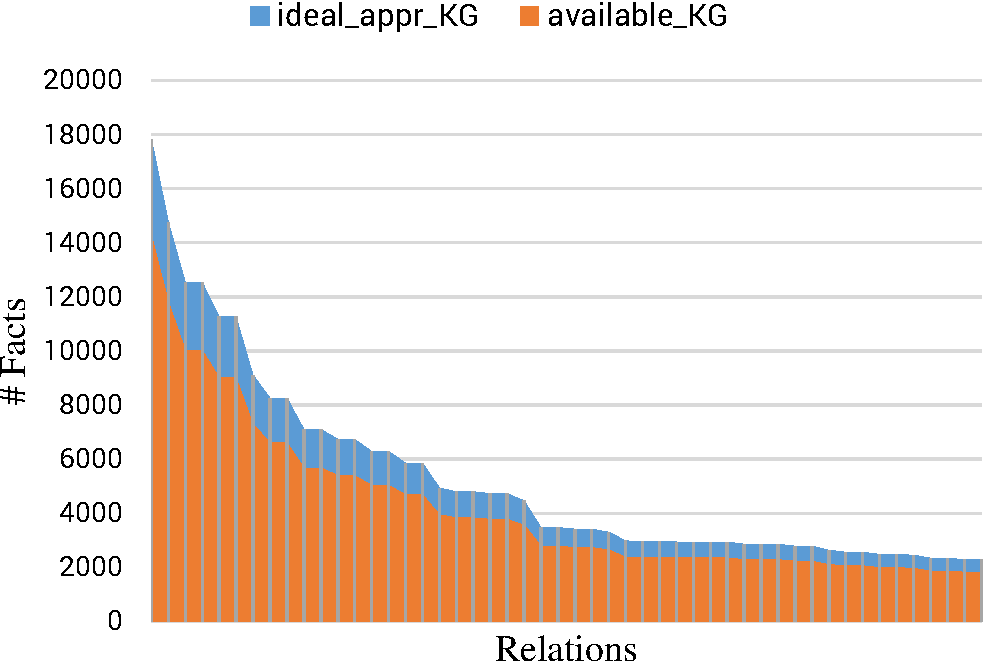
\includegraphics[width=0.5\textwidth]{figures/technical_rp/fb15k_pred_dist-crop.pdf} }}
     \subfloat[Wiki44K]{{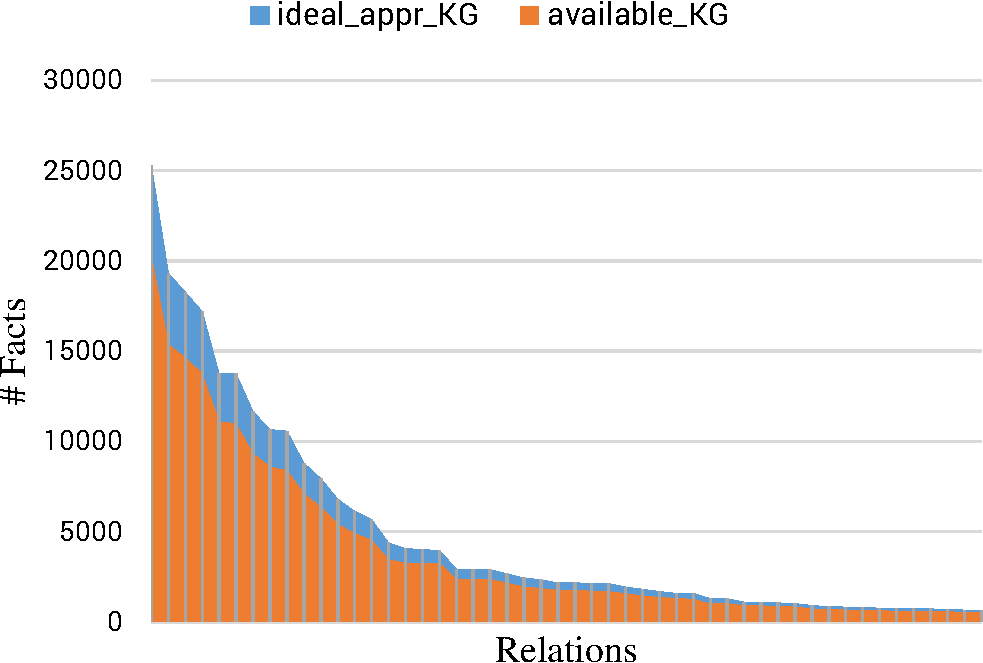
\includegraphics[width=0.5\textwidth]{figures/technical_rp/wiki44k_pred_dist-crop.pdf} }}\\
     \subfloat[IMDB]{{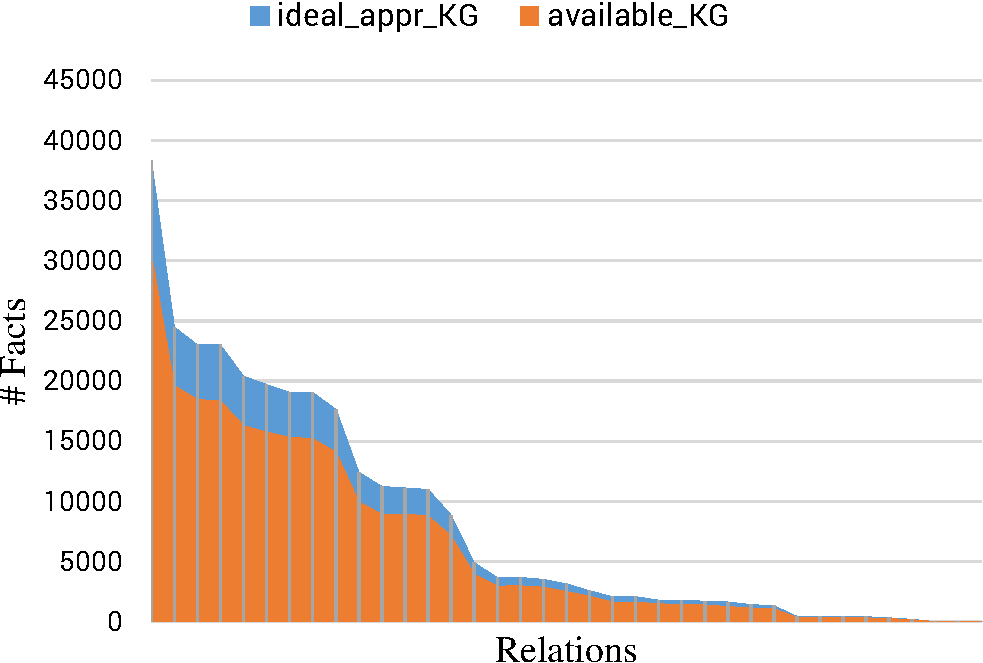
\includegraphics[width=0.5\textwidth]{figures/technical_rp/imdb_pred_dist-crop.pdf} }}
     \caption{Distribution of facts over top 50 relations of ideal approximation KG $\cG^i_{appr}$ and available KG $\cG$.}
     \label{table:pred_distribution}
\end{figure}

\begin{table}[h]
\centering
\begin{tabular}{ | l | l | } 
 \hline
 MODEL & NUMBER OF PARAMETERS \\ 
 \hline
 RESCAL\cite{conf/icml/NickelTK11} & $O(n_ek +n_rk^2)$    \\ 
 SE\cite{Bordes:2011:LSE:2900423.2900470} & $O(n_ek +2n_rk^2)$ \\ 
 SME(Linear)\cite{DBLP:journals/corr/abs-1301-3485} & $O(n_ek +n_rk +4k^2)$  \\ 
 SME(Bilinear)\cite{DBLP:journals/corr/abs-1301-3485} &  $O(n_ek +n_rk +2k^3)$ \\ 
 LFM \cite{Jenatton:2012:LFM:2999325.2999488} &  $O(n_ek +n_rk +10k^2)$ \\
 \hline
 TransE \cite{Bordes:NIPS2013} & $O(n_ek +n_rk)$  \\ 
 HolE\cite{DBLP:conf/aaai/NickelRP16} & $O(n_ek +n_rk)$  \\ 
 \hline
 SSP \cite{DBLP:conf/aaai/0005HMZ17} & $O(2n_ek +n_rk)$\\
 \hline
\end{tabular}
\newline
\caption{Numbers of parameters for some embedding models (Adapt from \cite{Bordes:NIPS2013}). $n_e$ and $n_r$ are the number of entities and binary predicates; $k$ is the embeddings dimension.}
\label{table:embedding_recap}
\vspace*{-3mm}
\end{table}
\leanparagraph{Embedding models}
Table \ref{table:embedding_recap} recaps some embedding models having been introduced in the literature and their memory complexity. TransE \cite{Bordes:NIPS2013} and HolE \cite{DBLP:conf/aaai/NickelRP16} are two state-of-the-art embedding models regarding the setting of no external data. Meanwhile, when talking about embedding models using additional texts, SSP \cite{DBLP:conf/aaai/0005HMZ17} plays an important part. Apart from prediction quality, these models also have a good running time and memory complexity. Hence, we choose them to evaluate our approach.
\begin{table}[t]
\scriptsize
\centering
\begin{tabular}{|l|r r|r r|r r|r r|} 
 \hline
 DATASET & \multicolumn{4}{|c|}{FB15K} & \multicolumn{4}{|c|}{WIKI44}\\
 \hline
 MODEL & \multicolumn{2}{|c|}{MRR}& \multicolumn{2}{|c|}{Hits@10(\%)} & \multicolumn{2}{|c|}{MRR}& \multicolumn{2}{|c|}{Hits@10(\%)} \\
 $Eval.\ setting$ & $Raw$ & $Filt.$ & $Raw$ & $Filt.$ & $Raw$ & $Filt.$ & $Raw$ & $Filt.$\\
 \hline
 TransE& 0.23 & 0.33 & 47.48 & 59.64 & 0.22 & 0.26 & 39.23 & 43.58\\
 HolE & 0.24 & 0.36 & 47.54 & 60.45& 0.14 & 0.18 & 24.54 & 28.38  \\
 SSP & 0.29 & \textbf{0.45}& 55.73 & \textbf{70.35}& 0.26 & \textbf{0.31} & 45.15 & \textbf{51.05} \\
 \hline
\end{tabular}
\caption{Performance of embedding models on the two data sets.}
\label{table:embedding_performance}
\vspace*{-3mm}
\end{table}

We train these embedding models on the available KG $\cG$ of these datasets until convergence using Stochastic Gradient Descent. For evaluation protocol of the embedding models, we use the same method as in HolE \cite{DBLP:conf/aaai/NickelRP16}. To validate and test the models, we sampled 2000 facts from $\cG^i_{appr} \setminus \cG$ into the validation set, and other 2000 facts into the test set. We report the Mean Reciprocal Rank and the percentage of Hit@10 in Table \ref{table:embedding_performance}. The optimal hyperparameters  of each model and dataset are figured out by doing grid search. We select the hyperparameters, which result in the highest MRR score with \textit{filtered} setting on the validation set. To get a better understanding about how the evaluation is performed, see \cite{DBLP:conf/aaai/NickelRP16}.

\subsection{Embedding-Based Hybrid Quality Function}
\begin{figure}[t]
     \centering
     \subfloat[Conf-TransE on IMDB]{{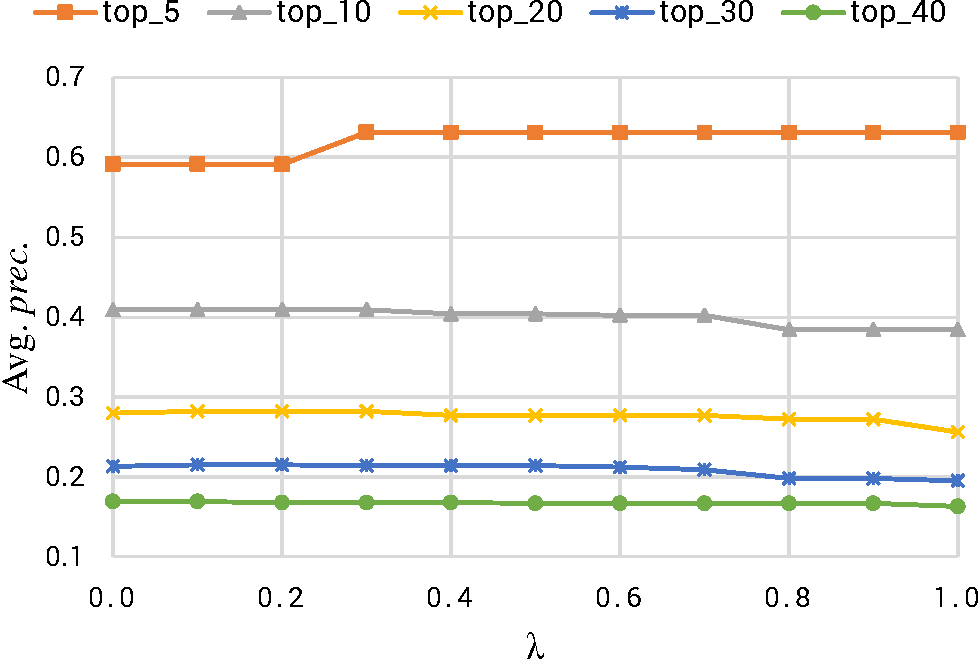
\includegraphics[width=0.5\textwidth]{figures/technical_rp/imdb_transe_conf-crop.pdf} }}
     \subfloat[Conv-TransE on IMDB]{{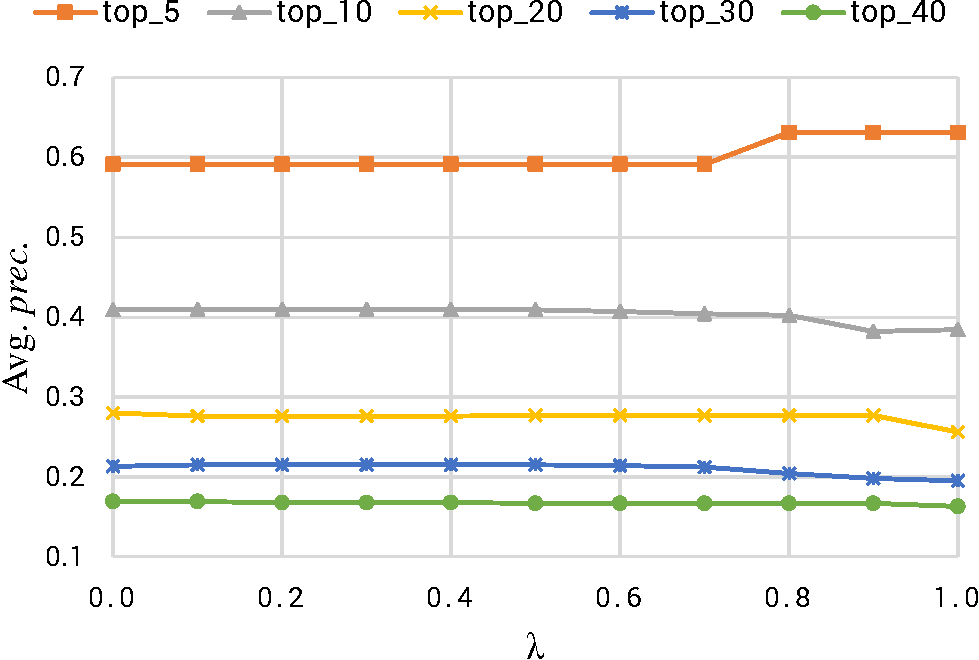
\includegraphics[width=0.5\textwidth]{figures/technical_rp/imdb_transe_conv-crop.pdf} }}\\
     \subfloat[PCA-TransE on IMDB]{{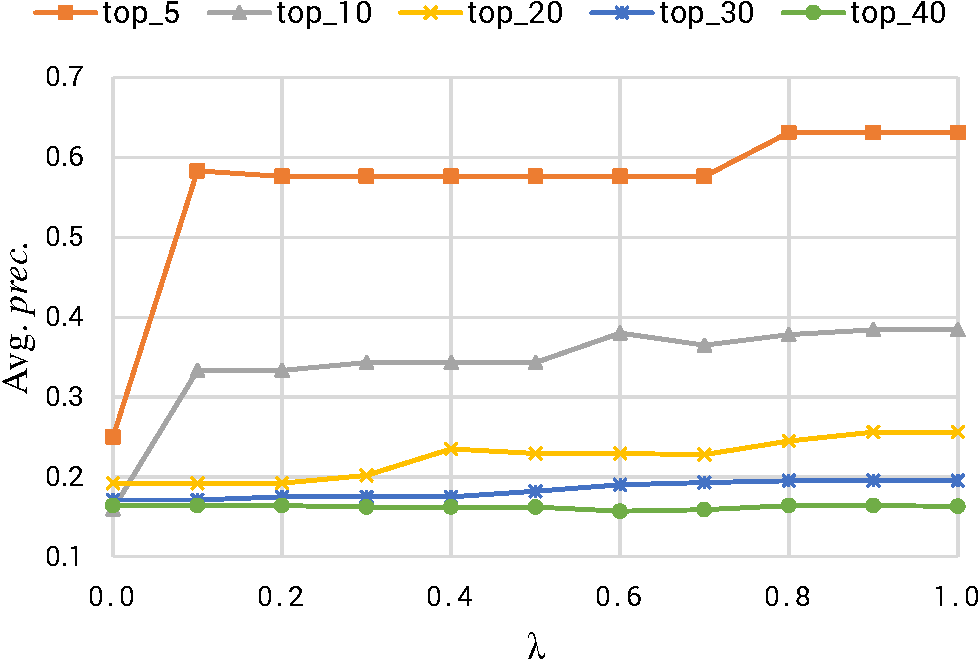
\includegraphics[width=0.5\textwidth]{figures/technical_rp/imdb_transe_pca-crop.pdf} }}
     \caption{$pred\_prec_{CW}$ of the \textit{top-k} rules with various \textit{embedding weights} on IMDB dataset.}
     \label{fig:appendix_exp1_imdb}
\end{figure}

Tables \ref{fig:appendix_exp1_imdb}, \ref{fig:appendix_exp1_fb15k}, \ref{fig:appendix_exp1_wiki44k} demonstrates the evaluation for experiment 1 for 3 mentioned datasets, with different configs, where we use $conf$, $conf_{pca}$ as $\mu_1$ and use TransE, HolE and SSP models to compute $\mu_2$. In addition, even though we require $\mu_1 \in [0,1]$, we also want to try one other metric, which does not hold this condition, to realize $\mu_1$. The metric we choose is $conviction$ \cite{trantowards}. Given $\mi{r:\; head\leftarrow body^+, not\;  body^-}$, conviction of $r$ is computed as follows:
\begin{align*}
\textit{conv}(r,\cG) & := \frac{1 - \textit{rel-supp}(head, \cG)}{1-\textit{conf}(r,\cG)}
\end{align*}
where $\textit{rel-supp}(head)$ is the relative support of the head, which is measured by:
\begin{align*}
\textit{rel-supp}(head, \cG) = \frac{|\set{(h, t) \mid head(h,t) \in \cG}|}{|\set{h \mid \exists t' \text{ s.t. }head(h,t') \in \cG}| \times |\set{t \mid \exists h'\text{ s.t. } head(h',t) \in \cG}|}
\end{align*}

We can see that with $conviction$, the best value of embedding weight $\lambda$ is close to 1. This is reasonable, since conviction could give us a value greater than 1. In addition, on \textit{IMDB} dataset, the usage of our hybrid quality measure does improve the quality of result. However, the improvement is not easily noticeable. One explanation is that this dataset is very spare, which could lead to the ineffectiveness of the embedding models.
\begin{figure}[t]
     \centering
     \subfloat[Conf-HoLE on FB15K]{{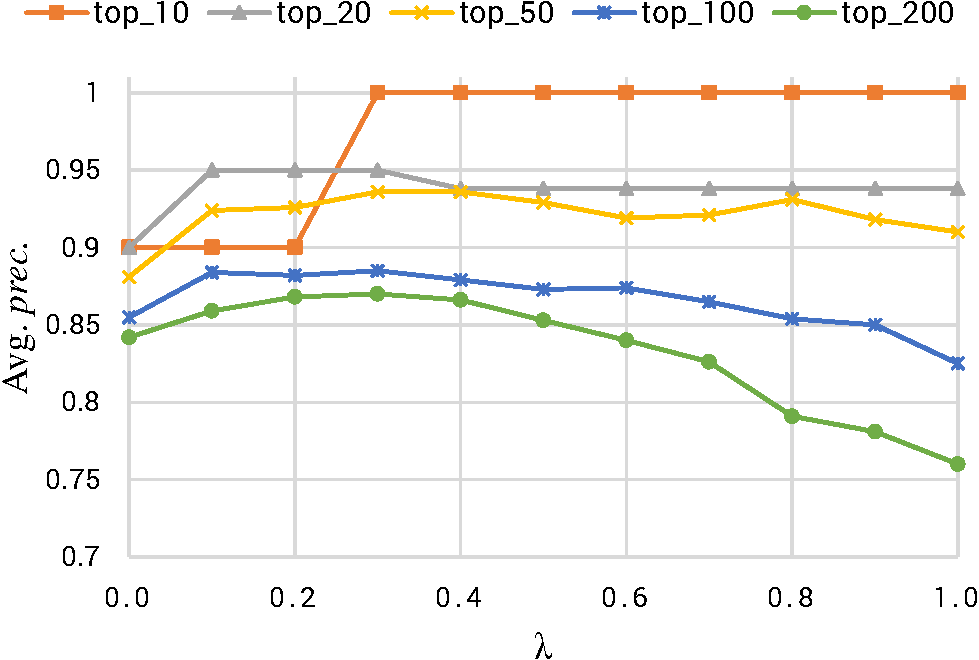
\includegraphics[width=0.5\textwidth]{figures/technical_rp/fb15k_hole_conf-crop.pdf} }}
     \subfloat[Conf-SSP on FB15K]{{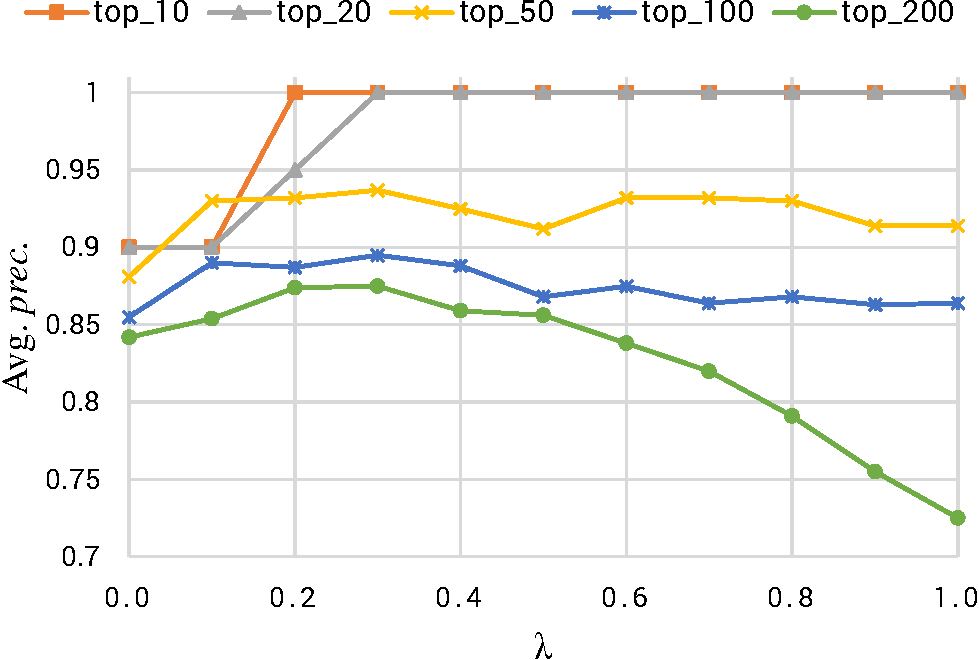
\includegraphics[width=0.5\textwidth]{figures/technical_rp/fb15k_ssp_conf-crop.pdf}}}\\
     \subfloat[PCA-HolE on FB15K]{{\includegraphics[width=0.5\textwidth]{figures/technical_rp/fb15k_hole_pca-crop.pdf} }}
     \subfloat[PCA-SSP on FB15K]{{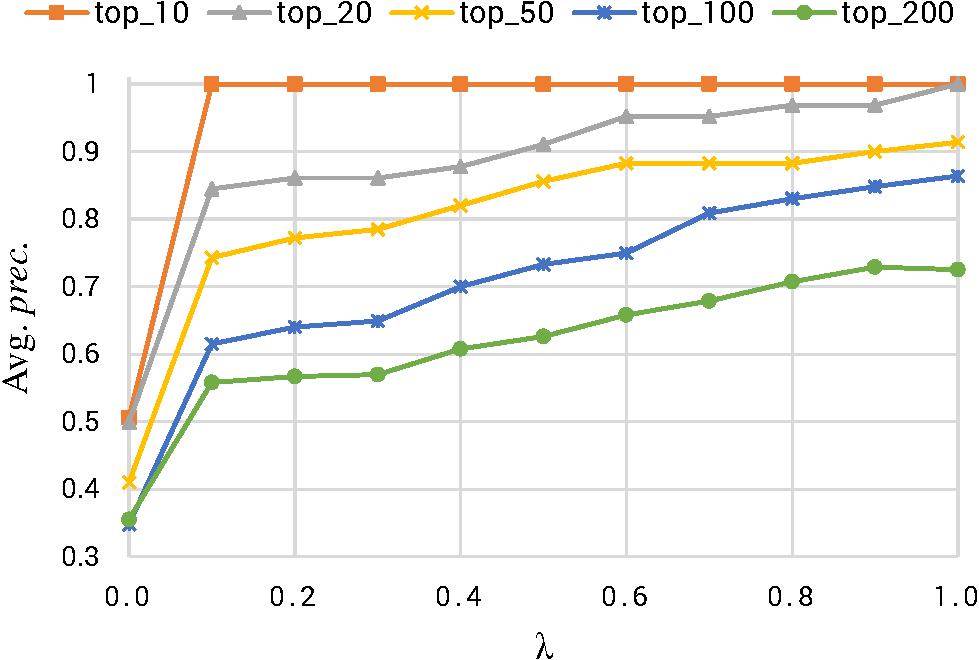
\includegraphics[width=0.5\textwidth]{figures/technical_rp/fb15k_ssp_pca-crop.pdf} }} \\   
     \subfloat[Conv-HolE on FB15K]{{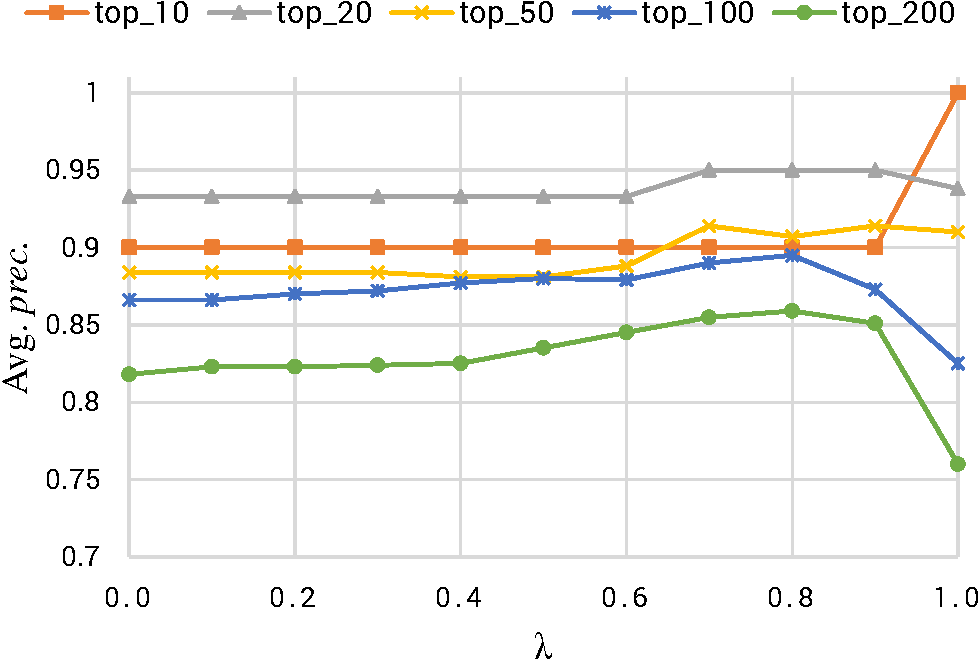
\includegraphics[width=0.5\textwidth]{figures/technical_rp/fb15k_hole_conv-crop.pdf} }}
     \subfloat[Conv-SSP on FB15K]{{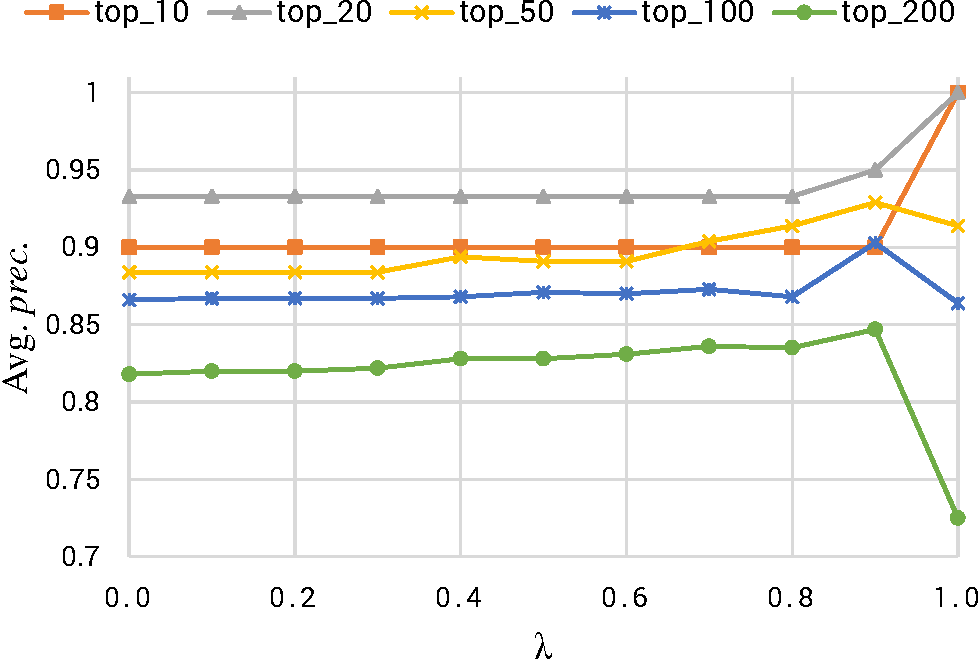
\includegraphics[width=0.5\textwidth]{figures/technical_rp/fb15k_ssp_conv-crop.pdf} }} \\   
     \caption{$pred\_prec_{CW}$ of the \textit{top-k} rules with various \textit{embedding weights} on FB15K dataset.}
     \label{fig:appendix_exp1_fb15k}
\end{figure} 
\begin{figure}[t]
     \centering
     \subfloat[Conf-TransE on Wiki44K]{{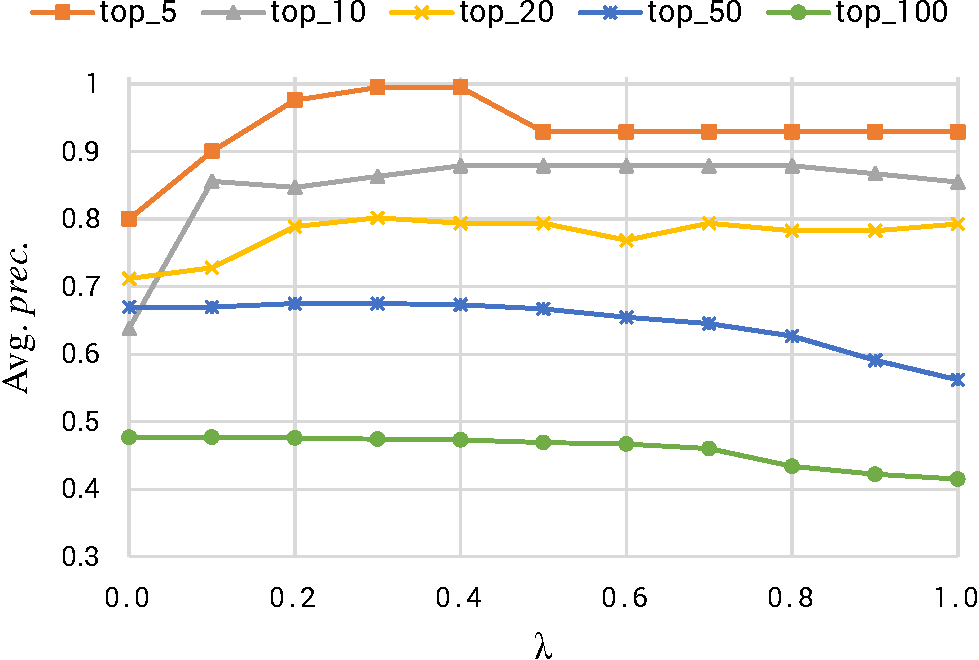
\includegraphics[width=0.5\textwidth]{figures/technical_rp/wiki44k_transe_conf-crop.pdf} }}
     \subfloat[Conf-SSP on Wiki44K]{{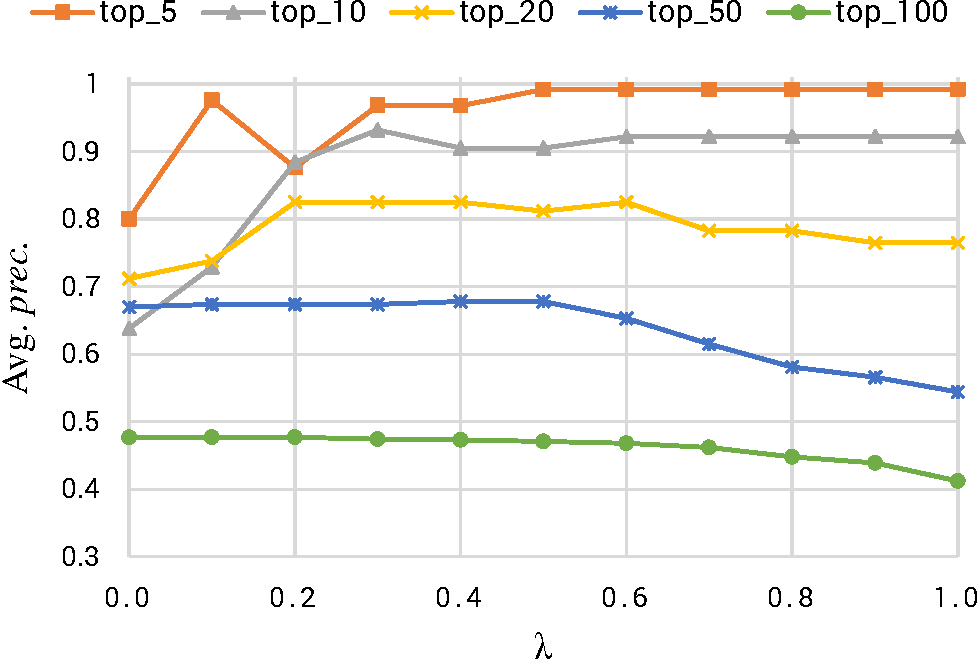
\includegraphics[width=0.5\textwidth]{figures/technical_rp/wiki44k_ssp_conf-crop.pdf}}}\\
     \subfloat[PCA-TransE on Wiki44K]{{\includegraphics[width=0.5\textwidth]{figures/technical_rp/wiki44k_transe_pca-crop.pdf} }}
     \subfloat[PCA-SSP on Wiki44K]{{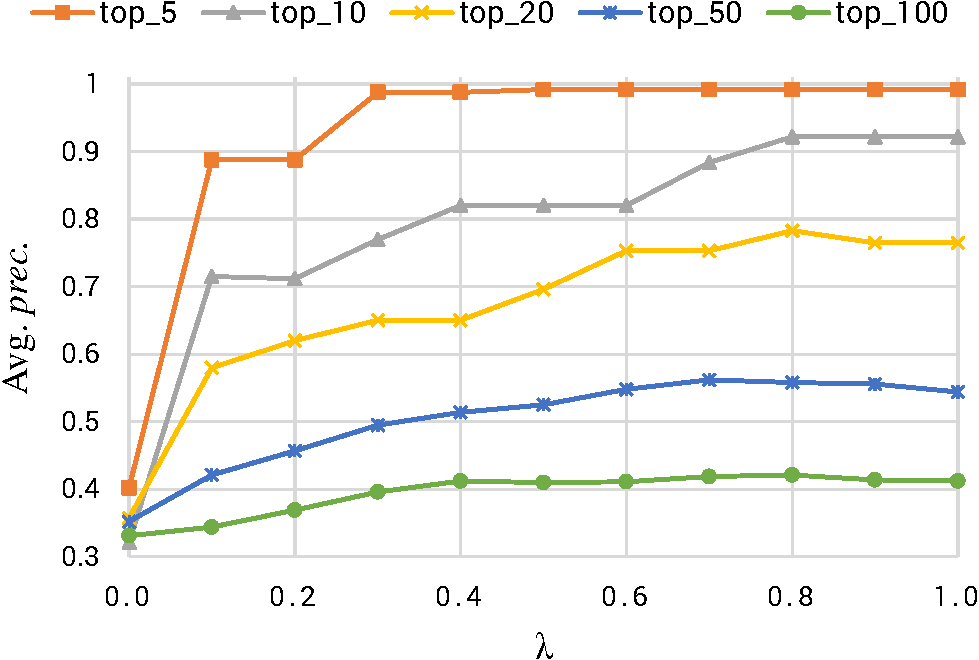
\includegraphics[width=0.5\textwidth]{figures/technical_rp/wiki44k_ssp_pca-crop.pdf} }} \\   
     \subfloat[Conv-TransE on Wiki44K]{{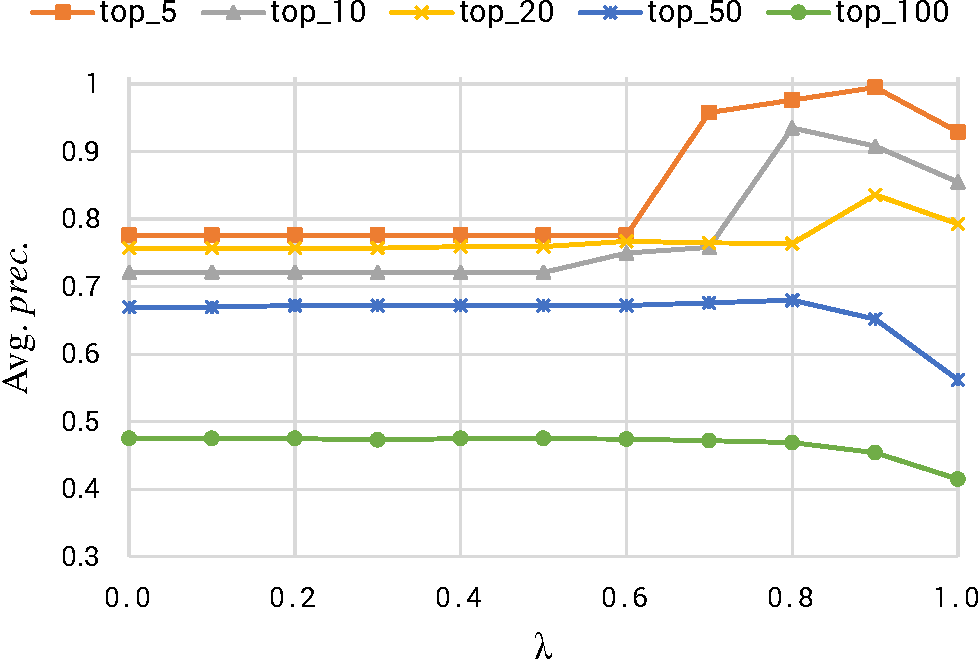
\includegraphics[width=0.5\textwidth]{figures/technical_rp/wiki44k_transe_conv-crop.pdf} }}
     \subfloat[Conv-SSP on Wiki44K]{{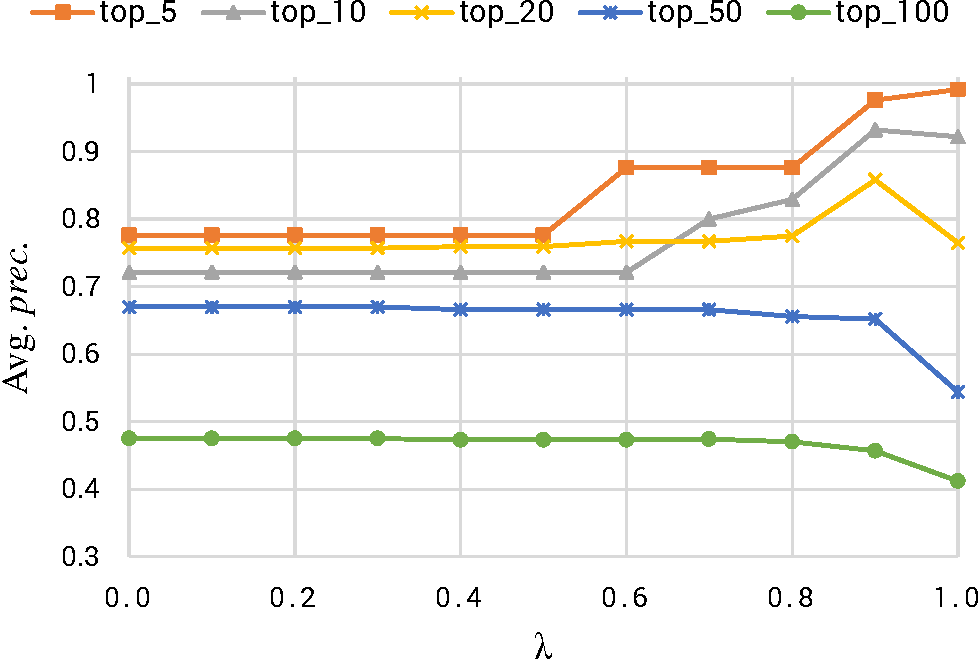
\includegraphics[width=0.5\textwidth]{figures/technical_rp/wiki44k_ssp_conv-crop.pdf} }}\\   
     \caption{$pred\_prec_{CW}$ of the \textit{top-k} rules with various \textit{embedding weights} on Wiki44K dataset.}
     \label{fig:appendix_exp1_wiki44k}
\end{figure} 

\begin{figure}[t]
     \centering
     \subfloat[FB15K]{{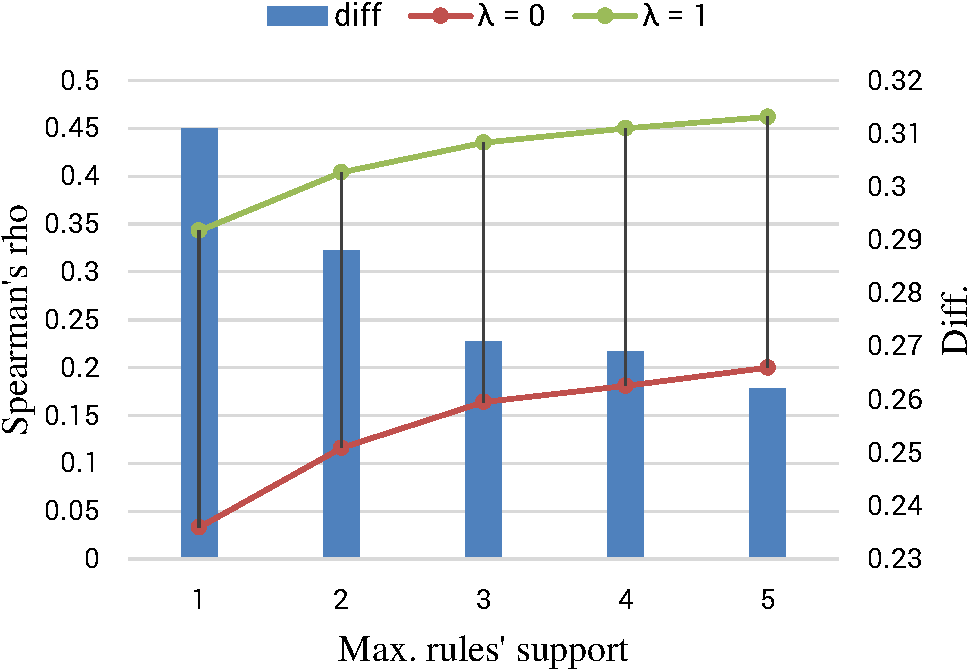
\includegraphics[width=0.5\textwidth]{figures/technical_rp/low_sp_fb15k-crop.pdf} }}
     \subfloat[Wiki44K]{{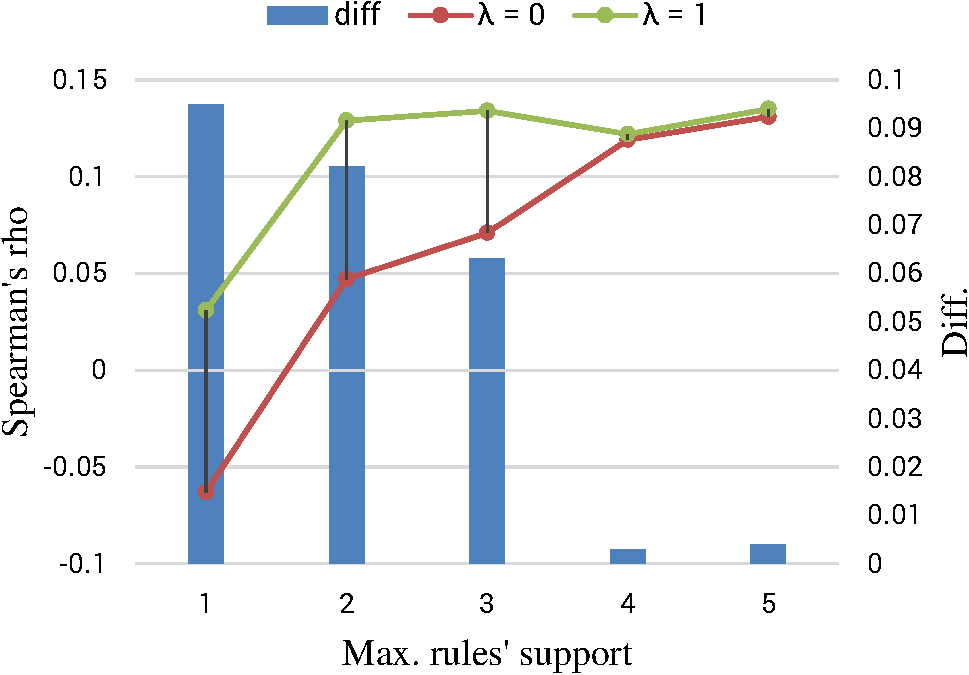
\includegraphics[width=0.5\textwidth]{figures/technical_rp/low_sp_wiki44k-crop.pdf} }}\\
     \subfloat[IMDB]{{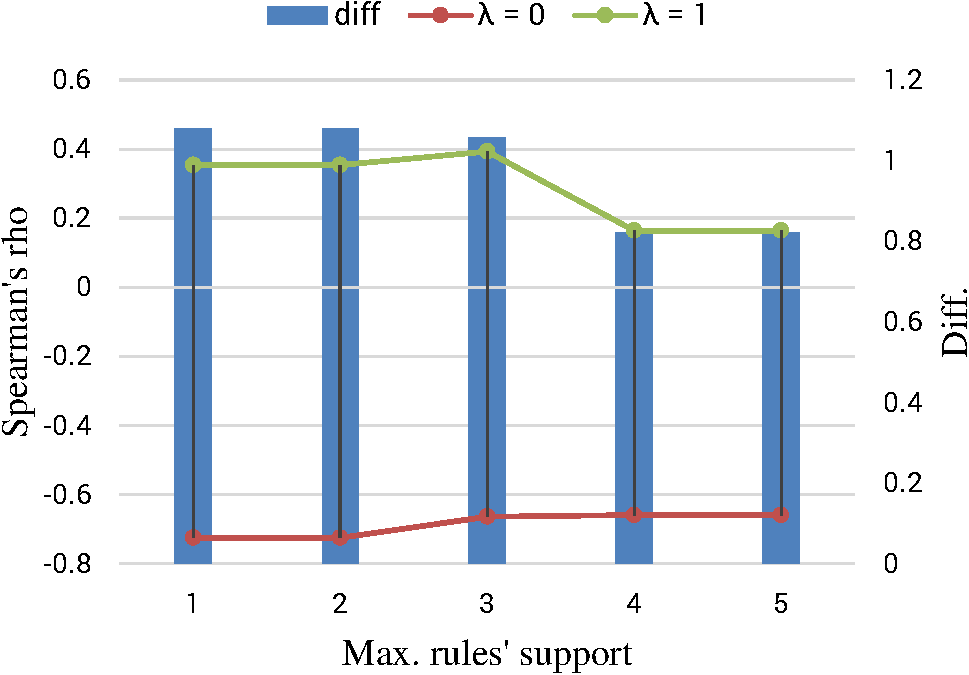
\includegraphics[width=0.5\textwidth]{figures/technical_rp/low_sp_imdb-crop.pdf} }}
     \caption{Spearman's rho of top rules ranked by confidence and the hybrid quality function, with limit on rules' support.}
     \label{fig:low_sp}
\end{figure}
\subsubsection{Handling rules with low support.}
One advantage of using the hybrid quality function comparing to standard rule measures (e.g. standard confidence) is at assessing rules having low support. In particular, when the rules have very low support, standard confidence is unreliable, since it estimates the rules' quality based on only a very small number of rules' instances. For example, ignoring all rules having confidence 1 since they do not infer any new facts, when a rule has support 1, its confidence is never greater than 0.5, even though the predicted facts may be good. 

Hybrid quality function $\mu$ fixes this issues by directly looking at the quality of predicted facts, which is achieved by feedback from the embedding models. We verify this hypothesis on \textit{FB15K}, \textit{Wiki44K} and \textit{IMDB} datasets. We also extracts rules of form $r:\;h(X,Z) \leftarrow p(X,Y), q(Y,Z)$ from $\cG$, with $conf(r,\cG) \geq 0.1$ and $\textit{r-supp}(r,\cG) \leq k$, where $k$ indicates the maximum support of rules to be extracted, we try different values of $k \in \{1,2,3,4,5\}$. These rules are then ranked using standard confidence itself ($\mu_1 = conf (\lambda = 0)$) and our hybrid quality function $\mu$. In addition, since we hypothesize that the confidence does not give strong information about the rules in this situation, we use $\mu = \mu_2 (\lambda = 1)$, where the hybrid quality function relies only on feedback from the embedding models. To compute $\mu_2$ in this case, we use the best embedding models for each dataset: SSP for \textit{FB15K}, \textit{Wiki44K} and TransE for \textit{IMDB}.

To evaluate the quality of the 2 ranked rule lists, we measure the Spearman's rank correlation coefficient of rules' confidence or hybrid quality with their $pred\_prec_{CW}$. Figure \ref{fig:low_sp} show the Spearman's rho of the 2 ranked lists and the difference of them with many values of rules support limit $k$. We can notice that the hybrid quality function outperforms standard confidence on all 3 datasets, and even works better with lower rule support.

\bibliographystyle{abbrv}
\bibliography{references}



\end{document}
